% USENIX-like two-column systems-paper layout.
% Hyperref / url / xcolor options must be set before the class line.
\PassOptionsToPackage{unicode}{hyperref}
\PassOptionsToPackage{hyphens}{url}
\PassOptionsToPackage{dvipsnames,svgnames,x11names}{xcolor}
\documentclass[letterpaper,10pt,twocolumn]{article}
\usepackage{xcolor}

% Geometry: 7 in x 9 in centered text block; 0.33 in column gutter.
\usepackage[
  letterpaper,
  textwidth=7in,
  textheight=9in,
  centering,
  columnsep=0.33in,
  headheight=14pt,
]{geometry}

% Math.
\usepackage{amsmath,amssymb,amsthm,mathtools}
\usepackage{newunicodechar}
\usepackage{fvextra}
\fvset{breaklines=true,breakanywhere=true,fontsize=\footnotesize,xleftmargin=0pt}
\newunicodechar{↾}{\ensuremath{\upharpoonright}}

% Paper-specific math macros (hybrid notation).
%
% PREDICATES / RELATIONS / CONSTRUCTORS render as short \mathsf{...}
% abbreviations (visual cue: this is a relation or constant).  Each
% abbreviation is introduced once in the \S5 notation table and
% spelled out in the surrounding prose where helpful.
%
% ACCESSOR FUNCTIONS (return a value) render as italic descriptive
% words via \mathit{...}.  Short, English, no underscores or hyphens
% inside math.  Reader can read the math directly as English: "apply
% prefix of R restricted to scope of R".
\newcommand{\restrict}{\mathbin{\upharpoonright}}
% Accessor functions (value-returning, italic):
\newcommand{\Apply}{\mathit{apply}}
\newcommand{\Src}{\mathit{src}}
\newcommand{\Scope}{\mathit{scope}}
\newcommand{\Frontier}{\mathit{frontier}}
\newcommand{\CleanPrefix}{\mathit{prefix}}
\newcommand{\Verify}{\mathit{verify}}
\newcommand{\AnchorDomain}{\mathit{anchorDom}}
\newcommand{\TouchedBetween}{\mathit{touched}}
\newcommand{\TableScopeBetween}{\mathit{tblScope}}
\newcommand{\ReplayKeys}{\mathit{keys}}
\newcommand{\Chunks}{\mathit{chunks}}
\newcommand{\SourceHistory}{\mathit{srcHistory}}
\newcommand{\CdcEvents}{\mathit{cdcEvents}}
% Variables / carriers (italic; not value-returning accessors).
% Rendered like accessors but carry external observations or
% schematic placeholders rather than computed values.
\newcommand{\RawObs}{\mathit{raw}}
\newcommand{\SinkState}{\mathit{sinkState}}
% Predicates / relations / constants (sans-serif abbreviations).
% Both the descriptive long-form macro names (\WellformedRun, ...) and
% short aliases (\WF, \FSO, ...) expand to the same compact
% \mathsf{...} symbol; either may be used in the body.
\newcommand{\WellformedRun}{\mathsf{WF}}
\newcommand{\WF}{\mathsf{WF}}
\newcommand{\FaithfulSourceObservation}{\mathsf{FSO}}
\newcommand{\FSO}{\mathsf{FSO}}
\newcommand{\MaterializesRun}{\mathsf{Mat}}
\newcommand{\Mat}{\mathsf{Mat}}
\newcommand{\CertRunCoherent}{\mathsf{Coh}}
\newcommand{\Coh}{\mathsf{Coh}}
\newcommand{\VirtualCut}{\mathsf{VC}}
\newcommand{\VC}{\mathsf{VC}}
\newcommand{\VirtualCutState}{\mathsf{VCS}}
\newcommand{\VCS}{\mathsf{VCS}}
\newcommand{\WholeTableClaimScope}{\mathsf{WTS}}
\newcommand{\WTS}{\mathsf{WTS}}
\newcommand{\ContSeg}{\mathsf{ContSeg}}
\newcommand{\Accept}{\mathsf{Accept}}
\newcommand{\Reject}{\mathsf{Reject}}
\newcommand{\Unsupported}{\mathsf{Unsupported}}
% Value tokens (roman; data-constructor values rather than predicates):
\newcommand{\None}{\mathrm{None}}

\setcounter{secnumdepth}{5}

% Font stack: newtx (Times-like serif + math); lmodern fallback.
\usepackage{iftex}
\ifPDFTeX
  \usepackage[T1]{fontenc}
  \usepackage[utf8]{inputenc}
  \usepackage{textcomp}
  \IfFileExists{newtxtext.sty}{%
    \usepackage{newtxtext}%
    \usepackage[varvw]{newtxmath}%
  }{\usepackage{lmodern}}
\else
  \usepackage{unicode-math}
  \defaultfontfeatures{Scale=MatchLowercase}
  \defaultfontfeatures[\rmfamily]{Ligatures=TeX,Scale=1}
  \usepackage{lmodern}
\fi
\IfFileExists{upquote.sty}{\usepackage{upquote}}{}
\IfFileExists{microtype.sty}{%
  \usepackage{microtype}%
  \UseMicrotypeSet[protrusion]{basicmath}%
}{}

% Paragraph rhythm: indented paragraphs, no big skip --- systems-paper style.
\setlength{\parindent}{1em}
\setlength{\parskip}{0pt plus 0.5pt}
\setlength{\emergencystretch}{3em}
\raggedbottom            % natural column depth; avoids two-column flush-bottom glue stretching

% Hard rule: at most one float (figure*/figure/table*/table) per page.
% LaTeX's defaults (topnumber=2, dbltopnumber=2, totalnumber=3) would
% otherwise allow two wide floats to stack at the top of a page (e.g.,
% Figure 1 + Table 1 doubling up on page 3), which reads as
% float-crowding.  Setting all four placement-count counters to 1
% enforces the one-float-per-page invariant at the kernel level.
\setcounter{topnumber}{1}
\setcounter{bottomnumber}{1}
\setcounter{totalnumber}{1}
\setcounter{dbltopnumber}{1}

% Tables (two-column safe).  No longtable: it does not float and conflicts
% with two-column body.  Wide tables use table* + tabularx + booktabs.
\usepackage{booktabs,array,tabularx,ragged2e}
\newcolumntype{Y}{>{\RaggedRight\arraybackslash}X}
\providecommand{\tightlist}{\setlength{\itemsep}{0pt}\setlength{\parskip}{0pt}}

% Tight lists for narrow columns.
\usepackage{enumitem}
\setlist{topsep=2pt,partopsep=0pt,parsep=2pt,itemsep=2pt,leftmargin=*}

% Slightly more generous tolerances for two-column line-breaking.
\tolerance=1500
\hbadness=2000

% Bibliography.
\usepackage[numbers,sort&compress]{natbib}

% Float barrier (avoid float pile-ups on the same page).
\usepackage{placeins}

% Section headers: prevent automatic hyphenation.  Article-class default
% lets LaTeX hyphenate mid-word in section / subsection titles when a
% title doesn't fit on one line (e.g., "Vir-/tual" or "Re-/striction").
% raggedright on headings, plus maxed hyphenation penalties, leaves each
% title-word intact and wraps as whole tokens instead.  Headings are
% already left-aligned in the article class, so raggedright is a visual
% no-op for fitting titles and only relaxes justification when wrapping.
\usepackage{sectsty}
\allsectionsfont{\raggedright\hyphenpenalty=10000\exhyphenpenalty=10000}

% Citation-order bibliography: the DBLog paper (andreakis2020dblog)
% is cited first, in the Abstract, so unsrtnat puts it at position
% [1]; the Netflix Tech Blog post (dblog_netflix_blog), first cited
% in the Introduction, lands at [4] after the Abstract's Debezium
% and Flink CDC citations.  natbib is loaded with the [numbers]
% option above, so in-text \citep renders numerically ("[1]"),
% not author-year.
\bibliographystyle{unsrtnat}

% Hyperref (load late) + URL hygiene.
\usepackage{bookmark}
\IfFileExists{xurl.sty}{\usepackage{xurl}}{}
\urlstyle{same}
% Allow more flexible URL breaks in narrow 2-column layout (avoid hanging URLs).
% Stretch between URL atoms; xurl already provides /, ., -, ?, = break-points.
\Urlmuskip=0mu plus 1mu\relax
% Extend hyphenation penalty for URLs so xurl breaks at slashes/dots, not mid-letter.
\renewcommand{\UrlBreaks}{\do\.\do\@\do\/\do\\\do\!\do\_\do\|\do\;\do\>\do\]%
  \do\)\do\,\do\?\do\&\do\=\do\#\do\:\do\-\do\~\do\'%
  \do\+\do\(\do\[\do\{\do\}\do\<\do\"\do\*\do\$\do\%}
\hypersetup{
  pdftitle={A Theoretical Study of DBLog: Certified Virtual Cuts for a Snapshot-Equivalent Replay of Live Databases},
  pdfauthor={Andreas Andreakis},
  hidelinks}

% ------------------------------------------------------------------
% Figure-rendering stack (Set A figures, original development source
% at paper/figures/set_a_architectural/fig0{1..5}_*/figXX.tex; the
% live build-input copies are at figures/fig0{1..5}_*/figXX.tex
% next to this file).
% ------------------------------------------------------------------
\usepackage[normalem]{ulem}
\usepackage{tikz}
\usetikzlibrary{arrows.meta,decorations.pathreplacing,decorations.markings,%
                positioning,calc,shapes.geometric,shapes.misc,fit,%
                backgrounds,patterns,matrix,quotes}

% Shared palette + tikzset, used by all five figures.
\definecolor{gDark}{HTML}{3A3A3A}
\definecolor{gMid}{HTML}{6A6A6A}
\definecolor{gLight}{HTML}{A6A6A6}
\definecolor{gPale}{HTML}{E5E5E5}
\definecolor{gBg}{HTML}{F4F4F4}

\tikzset{
  setA/.style={
    font=\sffamily\footnotesize,
    every node/.style={inner sep=2.5pt, outer sep=0pt},
    >={Latex[length=4pt, width=3pt]},
    line cap=round, line join=round,
    line width=0.5pt,
  },
  block/.style={
    draw=gDark, line width=0.5pt, rounded corners=1pt,
    fill=white, align=center, inner sep=4pt,
  },
  blockFill/.style={block, fill=gPale},
  blockEmph/.style={block, line width=0.8pt},
  blockGhost/.style={
    draw=gLight, line width=0.4pt, rounded corners=1pt,
    fill=white, dashed, align=center, inner sep=4pt, text=gMid,
  },
  layerChip/.style={
    draw=gDark, line width=0.5pt, rounded corners=2pt,
    fill=gPale, minimum width=11mm, minimum height=8mm,
    font=\sffamily\bfseries\small, align=center, inner sep=2pt,
  },
  layerChipGhost/.style={
    layerChip, draw=gLight, fill=white, text=gMid,
    font=\sffamily\small,
  },
  axisLine/.style={-{Latex[length=3.2pt, width=2.4pt]}, gDark, line width=0.45pt},
  axisTick/.style={gDark, line width=0.45pt},
  flow/.style={-{Latex[length=3.5pt, width=2.6pt]}, gDark, line width=0.45pt},
  depFlow/.style={-{Latex[length=3.5pt, width=2.6pt]}, gMid, line width=0.45pt},
  weakFlow/.style={-{Latex[length=3.5pt, width=2.6pt]}, gLight, line width=0.4pt, dashed},
  guide/.style={gMid, line width=0.4pt, dotted},
  cutLine/.style={gDark, line width=1.4pt},
  brace/.style={decorate, decoration={brace, amplitude=3pt, raise=1pt}, gDark, line width=0.4pt},
  braceMirror/.style={decorate, decoration={brace, mirror, amplitude=3pt, raise=1pt}, gDark, line width=0.4pt},
  pill/.style={
    draw=gDark, line width=0.4pt, rounded corners=2pt,
    fill=white, inner xsep=3pt, inner ysep=1.5pt, align=center,
    font=\sffamily\scriptsize,
  },
  pillFill/.style={pill, fill=gPale},
  lane/.style={gMid, line width=0.35pt},
  sublabel/.style={font=\sffamily\scriptsize, text=gDark},
  sublabelDim/.style={font=\sffamily\scriptsize\itshape, text=gMid},
}

% ------------------------------------------------------------------
% Two-column title block.
% ------------------------------------------------------------------
\title{A Theoretical Study of DBLog}
\newcommand{\papersubtitle}{Certified Virtual Cuts for a Snapshot-Equivalent Replay of Live Databases}
\newcommand{\paperauthor}{Andreas Andreakis}

\makeatletter
\renewcommand{\maketitle}{%
  \twocolumn[{%
    \begin{center}
      {\LARGE\bfseries \@title\par}
      \vspace{0.35em}
      {\large \itshape \papersubtitle\par}
      \vspace{1.1em}
      {\large \paperauthor\par}
    \end{center}
    \vspace{1.5em}
  }]%
  \thispagestyle{plain}%
}
\makeatother
\author{}
\date{}

\begin{document}
\maketitle

% --- LAYOUT INVARIANT: SINGLE-COLUMN ABSTRACT ---
% The abstract block (this section plus the Keywords block, up to
% \section{Introduction}) MUST fit within the first (left) column on
% page 1.  It must NOT overflow into the second column, which is
% reserved for the start of section 1 (Introduction).
%
% After ANY edit to the abstract or keywords block:
%   1. Rebuild:  latexmk -pdf main.tex
%   2. Open the rendered PDF and visually verify page 1:
%        the right (second) column begins with "1 Introduction"
%        (or its body), NOT a continuation of the abstract.
%
% A failed check blocks the slice close.
% Codified at slice post-V332-abstract-single-column-restore (V-333)
% after V-319/V-326/V-328 silently pushed the abstract past the
% column boundary.  Binding: see DECISIONS.md D-057.
\section*{Abstract}\label{abstract}

This paper is a theoretical follow-up to the 2020 DBLog
paper~\citep{andreakis2020dblog}, which described a change-data-capture
(CDC) mechanism for backfilling a downstream system from a live
source database and streaming its ongoing changes, while the source
keeps accepting writes. DBLog reads the table in primary-key
range scans (chunks) interleaved with the source change log:
watermarks locate each chunk in log order, chunk rows become refresh
events, and CDC events repair stale chunk observations. The mechanism
requires no table lock, no pause in writes, and no global read
transaction, and is now adopted by
Debezium~\citep{debezium_incremental_snapshot} and Apache Flink
CDC~\citep{flink_cdc_incremental_snapshot}.

The 2020 paper described the mechanism operationally but did not
formalize its correctness object. This paper formalizes that object: DBLog constructs
a snapshot-equivalent replay certificate without requiring a single
physical snapshot read.

The central formal object is a \textbf{certified virtual cut}: a finite
evidence bundle whose certified replay reaches the same per-key state
as the source at a chosen frontier on a chosen key scope. A virtual cut
is extensional: replay equality at a frontier, not a physical snapshot
read, and asserts no single source timestamp across chunk rows. The
paper proves per-key replay equality for every wellformed DBLog run at
its frontier and scope, and that an accepted certificate, evaluated
against faithful source observation, witnesses such a run and yields a
virtual cut. It also proves two source-side algebra facts: on the
same scope, a cut advances to later frontiers by appending
the scope-filtered faithful CDC segment committed in between, and a cut
restricts to sub-scopes. Each
result is \emph{Conditional} on premises stated where it
appears. Whole-table correctness, exactly-once delivery, sink-state
convergence, and transfer to named deployments are not consequences of
certificate acceptance alone. All proofs are machine-checked in
Isabelle/HOL.

\smallskip
\noindent\textbf{Keywords.}\label{keywords}\enspace
databases, distributed systems, \mbox{online backfill},
change-data-capture, formal verification, Isabelle/HOL.

\section{Introduction}\label{introduction}

The DBLog change-data-capture (CDC) backfill mechanism was introduced
in the December 2019 Netflix Tech Blog
post~\citep{dblog_netflix_blog}; the 2020 DBLog
paper~\citep{andreakis2020dblog} followed, describing it
operationally: online primary-key chunk reads, watermarks bracketing
each chunk in the source log, refresh events derived from chunk rows,
ordinary CDC events filling the gaps, and stale refresh rows
suppressed when newer log evidence dominates them. DBLog-style
mechanisms have since shipped in
Debezium~\citep{debezium_incremental_snapshot} and Apache Flink
CDC~\citep{flink_cdc_incremental_snapshot}, where the chunk-based capture
phase this paper calls the \emph{backfill} is exposed as the
\emph{incremental snapshot}.

Live-source backfills are deceptively simple. A database operator wants
to copy a table, or a selected range of keys, into a downstream system
while the source keeps accepting writes. A direct physical snapshot
would give one clear answer: read the table at one database timestamp,
then replay changes after that timestamp. In many production settings
that is exactly what the operator is trying to avoid. Holding a
read transaction over a large table can be expensive; an interrupted
snapshot cannot be resumed and must restart in full; and a table lock
taken to read it consistently may block writes to the source.

DBLog-style backfills take a different route. They read the table in
primary-key chunks, observe the source log while those chunk reads
happen, and combine the two streams of evidence into a finite replay.
The chunk reads do not all occur at the same source-log coordinate.
Writes can land between them. Some chunk-read rows may already be stale
by the time the chosen frontier (the source-log coordinate the backfill
aims to match) is reached. The central question is therefore not
``which physical snapshot did DBLog read?'' but:

\begin{quote}
\itshape
Can the evidence DBLog gathered be replayed to the same per-key state as
the source at a chosen frontier on a chosen scope, and can that
replay-equivalence claim be advanced as the source commits later events?
\end{quote}

This paper answers that question extensionally. A \textbf{virtual cut}
is replay equality at a frontier on a scope. A \textbf{certified virtual
cut} is a virtual cut packaged behind a finite certificate and evidence
bundle: the replay prefix, the claimed scope, the claimed frontier, and
the source-side evidence needed to justify them.

A virtual cut is point-in-time, but it is not one-shot. DBLog's backfill
phase, the chunk loop, bootstraps the first certified virtual cut for
a scope and frontier; once the chunk loop closes, appending the source's
faithful change data advances that cut to later frontiers. Ongoing DBLog
operation is therefore a sequence of source-side replay-equivalence
claims, and this paper proves both the point-in-time equality and the
source-side continuation that links them.

The original publications named the mechanism, motivated its operational
shape, and argued informally that watermark bracketing together with
stale-row suppression yields a consistent capture of the chosen scope;
they did not state that consistency as a formal object, give it a
specification, or machine-check it. This paper supplies that
formalization through a layered theorem ladder; the watermark
mechanics themselves enter it as stated premises --- the
single-coordinate chunk-read attribution of
Section~\ref{watermarks-and-chunk-read-coordinates} --- not as
derived results. The ladder links wellformed DBLog
runs to accepted certificates evaluated against faithful source
observation, specializes the result to whole-table backfills, and
extends it through a source-side continuation that carries a cut to
later frontiers. Every theorem in the ladder is mechanically checked in
the companion formal development, archived on Zenodo at
\url{https://doi.org/10.5281/zenodo.20652511}. The paper is therefore a
theoretical study of an existing system: neither a re-introduction of
DBLog nor a product-verification claim about any named implementation.

The technical development is layered through the source-side core.
Figure~\ref{fig:theorem-ladder} separates that core ladder from the
post-core extension map. Layers~0 through~4 form the core dependency
ladder: the source and replay model, abstract DBLog runs, source-side
virtual-cut soundness, accepted-certificate soundness, and the
whole-table specialization.

\begin{figure*}[t]
  % fig01.tex -- Set A (Architectural) Figure 1: theorem ladder + post-core extension map.

\centering
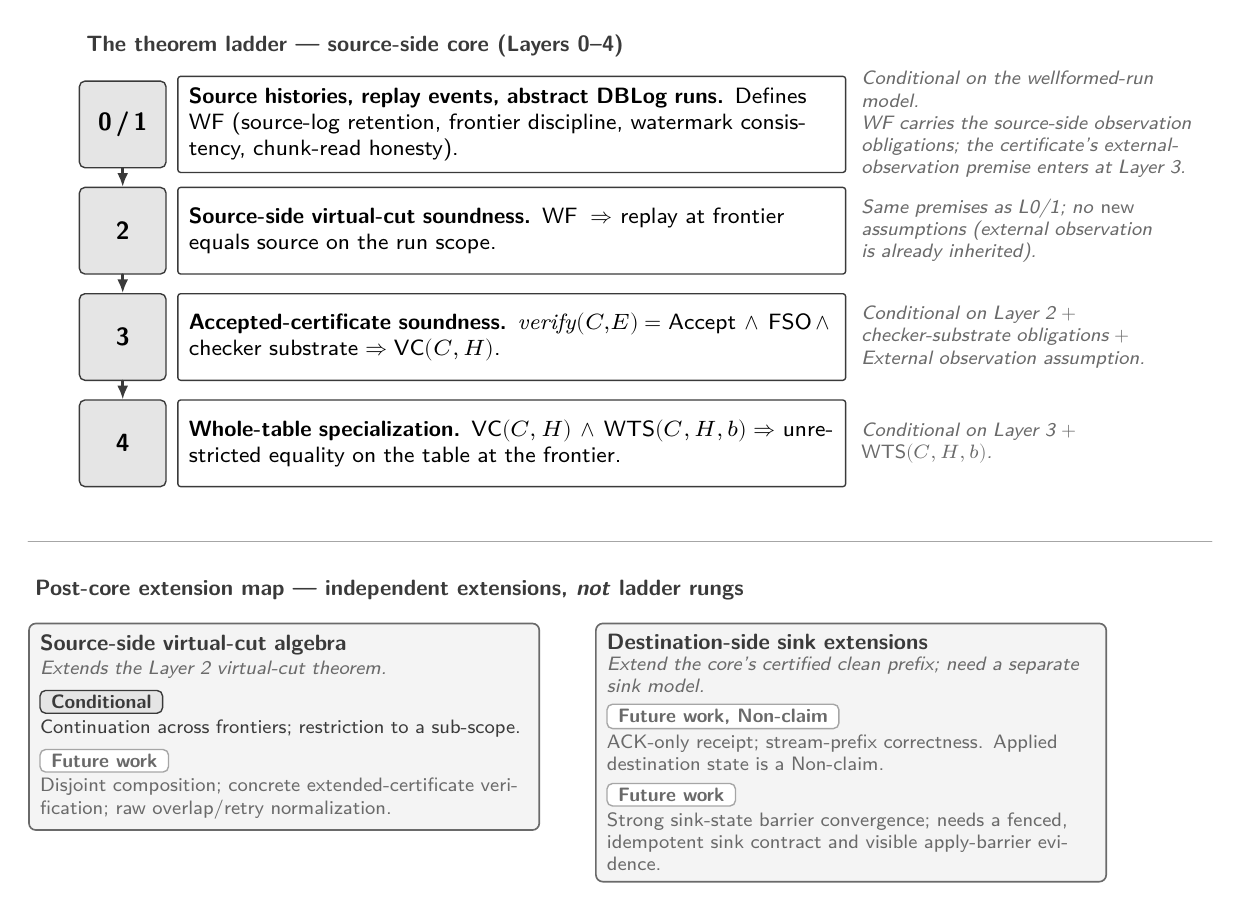
\begin{tikzpicture}[setA]

% ============================================================
% Styles.
%   Panel A (the core ladder): chip + slab + premise note.
%   Panel B (the post-core extension map): titled cards with
%   per-item status chips.
% ============================================================
\tikzset{
  ladderChip/.style={layerChip, minimum width=11mm, minimum height=11mm},
  ladderSlab/.style={block, text width=82mm, minimum height=11mm,
                     align=left, inner sep=4pt, font=\sffamily\footnotesize},
  ladderNote/.style={font=\sffamily\scriptsize\itshape, text=gMid,
                     text width=44mm, align=left, anchor=west,
                     inner sep=0pt},
  panelHd/.style={font=\sffamily\bfseries\footnotesize, text=gDark,
                  anchor=west},
  cardTtl/.style={font=\sffamily\bfseries\footnotesize, text=gDark,
                  anchor=north west, text width=62mm, align=left,
                  inner sep=0pt},
  cardAtt/.style={font=\sffamily\scriptsize\itshape, text=gMid,
                  anchor=north west, text width=62mm, align=left,
                  inner sep=0pt},
  cardTxt/.style={font=\sffamily\scriptsize, text=gDark,
                  anchor=north west, text width=62mm, align=left,
                  inner sep=0pt},
  cardTxtG/.style={font=\sffamily\scriptsize, text=gMid,
                   anchor=north west, text width=62mm, align=left,
                   inner sep=0pt},
  chipNow/.style={draw=gDark, line width=0.5pt, rounded corners=2pt,
                  fill=gPale, font=\sffamily\bfseries\scriptsize,
                  text=gDark, inner xsep=4pt, inner ysep=1.6pt,
                  anchor=north west},
  chipFut/.style={draw=gLight, line width=0.5pt, rounded corners=2pt,
                  fill=white, font=\sffamily\bfseries\scriptsize,
                  text=gMid, inner xsep=4pt, inner ysep=1.6pt,
                  anchor=north west},
  cardBox/.style={draw=gMid, line width=0.6pt, rounded corners=2.5pt,
                  fill=gBg},
}

\def\rowGap{2.5mm}

% ============================================================
% PANEL A -- the source-side core: the theorem ladder.
% Layers 0--4, each rung Conditional and depending on the rung
% above it.
% ============================================================
\node[panelHd] (hdA) at (-5.5mm,10mm)
  {The theorem ladder \textemdash\ source-side core (Layers 0--4)};

% --- LAYER 0/1 (two formal layers folded into one row) ---
\node[ladderChip] (c01) at (0,0) {0\,/\,1};
\node[ladderSlab,  right=1.5mm of c01, anchor=west] (s01) {%
  \textbf{Source histories, replay events, abstract DBLog runs.}
  Defines $\WellformedRun$ (source-log retention, frontier discipline,
  watermark consistency, chunk-read honesty).};
\node[ladderNote,  right=2mm   of s01]              (n01)                      {%
  Conditional on the wellformed-run model.\\
  WF carries the source-side observation\\
  obligations; the certificate's external-\\
  observation premise enters at Layer 3.};

% --- LAYER 2 ---
\node[ladderChip,  below=\rowGap of c01.south, anchor=north] (c2)              {2};
\node[ladderSlab,  right=1.5mm of c2,  anchor=west]          (s2)              {%
  \textbf{Source-side virtual-cut soundness.}
  $\WellformedRun \Rightarrow$ replay at frontier equals source on the
  run scope.};
\node[ladderNote,  right=2mm   of s2]                        (n2)              {%
  Same premises as L0/1; no \emph{new}\\
  assumptions (external observation\\
  is already inherited).};

% --- LAYER 3 ---
\node[ladderChip,  below=\rowGap of c2.south, anchor=north]  (c3)              {3};
\node[ladderSlab,  right=1.5mm of c3, anchor=west]           (s3)              {%
  \textbf{Accepted-certificate soundness.}
  $\Verify(C{,}E)=\Accept \,\land\, \FaithfulSourceObservation \,\land\,$
  checker substrate $\Rightarrow \VirtualCut(C, H)$.};
\node[ladderNote,  right=2mm   of s3]                        (n3)              {%
  Conditional on Layer 2 $+$\\
  checker-substrate obligations $+$\\
  External observation assumption.};

% --- LAYER 4 ---
\node[ladderChip,  below=\rowGap of c3.south, anchor=north]  (c4)              {4};
\node[ladderSlab,  right=1.5mm of c4, anchor=west]           (s4)              {%
  \textbf{Whole-table specialization.}
  $\VirtualCut(C, H) \,\land\, \WholeTableClaimScope(C, H, b) \Rightarrow$
  unrestricted equality on the table at the frontier.};
\node[ladderNote,  right=2mm   of s4]                        (n4)              {%
  Conditional on Layer 3 $+$\\
  $\WholeTableClaimScope(C, H, b)$.};

% Dependency spine: lower depends on upper.
\foreach \a/\b in {c01/c2, c2/c3, c3/c4} {
  \draw[-{Latex[length=5pt, width=4pt]}, gDark, line width=0.9pt]
    ([yshift=-0.2pt]\a.south)
    -- ([yshift=0.2pt]\b.north);
}

% ============================================================
% Panel divider -- a neutral layout rule. NOT a status boundary:
% the post-core area below is mixed-status, so no "future work"
% line is drawn.
% ============================================================
\coordinate (divL) at ($(c4.south west) + (-6.5mm, -7mm)$);
\coordinate (divR) at ($(n4.east |- divL) + (0.5mm, 0)$);
\draw[gLight, line width=0.4pt] (divL) -- (divR);

% ============================================================
% PANEL B -- the post-core extension map.
% Two independent extension paths off the core; NOT ladder
% rungs. Each card carries per-item status chips.
% ============================================================
\node[panelHd, anchor=north west] (hdB) at ($(divL) + (0,-4mm)$)
  {Post-core extension map \textemdash\ independent extensions, \emph{not} ladder rungs};

% --- Card 1: source-side virtual-cut algebra (extends Layer 2) ---
\node[cardTtl, anchor=north west] (a-ttl) at ($(hdB.south west) + (1.5mm,-3.5mm)$)
  {Source-side virtual-cut algebra};
\node[cardAtt, anchor=north west] (a-att) at ([yshift=-0.8mm]a-ttl.south west)
  {Extends the Layer~2 virtual-cut theorem.};
\node[chipNow, anchor=north west] (a-c1) at ([yshift=-1.5mm]a-att.south west)
  {Conditional};
\node[cardTxt, anchor=north west] (a-d1) at ([yshift=-0.8mm]a-c1.south west)
  {Continuation across frontiers; restriction to a sub-scope.};
\node[chipFut, anchor=north west] (a-c2) at ([yshift=-1.6mm]a-d1.south west)
  {Future work};
\node[cardTxtG, anchor=north west] (a-d2) at ([yshift=-0.8mm]a-c2.south west)
  {Disjoint composition; concrete extended-certificate verification;
   raw overlap/retry normalization.};

% --- Card 2: destination-side sink extensions (extend the certified prefix) ---
\node[cardTtl, anchor=north west] (b-ttl) at ($(a-ttl.north west) + (72mm,0)$)
  {Destination-side sink extensions};
\node[cardAtt, anchor=north west] (b-att) at ([yshift=-0.8mm]b-ttl.south west)
  {Extend the core's certified clean prefix; need a separate sink model.};
\node[chipFut, anchor=north west] (b-c1) at ([yshift=-1.5mm]b-att.south west)
  {Future work, Non-claim};
\node[cardTxtG, anchor=north west] (b-d1) at ([yshift=-0.8mm]b-c1.south west)
  {ACK-only receipt; stream-prefix correctness. Applied destination
   state is a Non-claim.};
\node[chipFut, anchor=north west] (b-c2) at ([yshift=-1.6mm]b-d1.south west)
  {Future work};
\node[cardTxtG, anchor=north west] (b-d2) at ([yshift=-0.8mm]b-c2.south west)
  {Strong sink-state barrier convergence; needs a fenced, idempotent
   sink contract and visible apply-barrier evidence.};

% Card background boxes (drawn behind the content).
\begin{scope}[on background layer]
  \node[cardBox, fit=(a-ttl)(a-att)(a-c1)(a-d1)(a-c2)(a-d2),
        inner sep=4pt] {};
  \node[cardBox, fit=(b-ttl)(b-att)(b-c1)(b-d1)(b-c2)(b-d2),
        inner sep=4pt] {};
\end{scope}

\end{tikzpicture}

\caption{Theorem ladder and post-core extension map. \textbf{Top
panel --- the source-side core.} Layers~0--4 form the core dependency
ladder: each layer is Conditional on the premises listed beside it
and on every layer above it. \textbf{Bottom panel --- the post-core
extension map}, \emph{not} a continuation of the ladder. The
source-side virtual-cut algebra card extends the Layer~2 virtual-cut
theorem: continuation across later frontiers is Conditional on that
theorem, a wellformed source history, and the faithful
continuation-segment premise, while restriction to a sub-scope is
Conditional only on an existing cut and a sub-scope inclusion;
disjoint composition, concrete
extended-certificate verification, and raw overlap/retry
normalization remain Future work. The destination-side sink
extensions extend the certified clean prefix the core produces but
require a separate sink model: ACK-only receipt and strong sink-state
barrier convergence are Future work, and applied destination-state
correctness is a Non-claim without a fenced, idempotent sink contract
and visible apply-barrier evidence. When a virtual cut is obtained
from an accepted certificate, the accepted-certificate premises and
the external observation assumption are inherited.}
\label{fig:theorem-ladder}

\end{figure*}

Beyond that core, the paper records independent extension paths rather
than further ladder rungs. The source-side virtual-cut algebra path
has two machine-checked Conditional results: continuation across
frontiers and restriction to a sub-scope
(Section~\ref{source-side-continuation-and-restriction}). The
remaining certificate-algebra program, disjoint composition,
concrete extended-certificate verification, and raw overlap/retry
normalization, remains Future work. The destination-side sink
path, covering ACK-only receipt and strong sink-state barrier
convergence, also remains Future work in this paper; applied
destination-state correctness is a Non-claim without a separate
fenced, idempotent sink contract and visible apply-barrier evidence.

The practitioner reading path is deliberately front-loaded. Section~2
walks a concrete backfill, and shows the cut advancing, before formal
notation appears. Section~3 names the DBLog mechanism in operational
terms. Section~4 states what
DBLog is, what it is not, and which failure modes matter. Section~8
can be read informally as the certificate and verifier vocabulary,
Section~\ref{source-side-continuation-and-restriction} records the
proved source-side continuation and restriction results, and
Section~\ref{sink-state-convergence-non-claim} records the sink-state
Non-claim. A theory reader can then follow Sections~5 through~11 for
the formal definitions, theorem statements, and proof explanations,
with Layers~0--4 forming the core ladder and
Section~\ref{source-side-continuation-and-restriction} the proved
post-core source-side algebra.

We use six status labels throughout
(Table~\ref{tab:status-vocab}):

\begin{table*}[t]
\caption{Reader-facing status vocabulary used throughout the paper.}
\label{tab:status-vocab}
\centering\small
\begin{tabularx}{\textwidth}{@{}lY@{}}
\toprule
\textbf{Status} & \textbf{Meaning in this paper}\\
\midrule
Proved &
  The claim is machine-checked, and the paper gives the proof idea or
  proof explanation in the body.\\
Conditional &
  The claim is proved under assumptions stated where the claim appears.\\
Deployment obligation &
  The operator or implementation must establish this condition in a
  deployment.\\
External observation assumption &
  The source-side observation is assumed faithful; the model cannot
  prove it from the certificate alone.\\
Future work &
  A named extension or theorem path that this paper does not claim.\\
Non-claim &
  A boundary: something the paper deliberately does not prove.\\
\bottomrule
\end{tabularx}
\end{table*}

This status vocabulary is part of the contribution. Every strong claim is
either proved under visible assumptions, assigned to the deployment,
marked as external observation, or explicitly kept outside the theorem.

\section{Bootstrapping and Advancing a Virtual Cut: A Running
Example}\label{bootstrapping-and-advancing-a-virtual-cut}

This section walks through one concrete scenario before any formal
definitions appear. It shows what DBLog gathers from a live source
database while concurrent writes are happening, how that material is
assembled into a replay, what it means for the replay to be
``equivalent to a snapshot'' without any single physical snapshot read
having taken place, and how the equivalence point advances as the
source keeps committing writes.

The same example is reused throughout the rest of the paper. The formal
model later in the paper makes every term in this section precise; here
we stay strictly operational.

\subsection{Setup}\label{setup}

A source database carries a single table:

\begin{center}\ttfamily\small
accounts(account\_id, balance)
\end{center}

with two live rows at the moment our story starts:

\begin{center}\footnotesize
\begin{tabular}{@{}l@{\hskip 1em}l@{\hskip 1em}l@{}}
\ttfamily account\_id = 100 & \ttfamily balance = \phantom{0}5000 & \itshape (Alice's account, \$50)\\
\ttfamily account\_id = 200 & \ttfamily balance = 10000           & \itshape (Bob's account, \$100)\\
\end{tabular}
\end{center}

A third user, Carol, has not yet opened an account; account\_id 300 does
not exist in the table.

A DBLog backfill is running concurrently with normal application
traffic. The application keeps writing to the source database while
DBLog reads chunks of rows and watches the source log. Our goal in the
example is to assemble the replay evidence for these accounts and to
show that replaying it has the same per-account outcome as the source at
one consistent point in time, even though no two reads happened at
exactly that same instant.

\subsection{What the Source Log Records During the Backfill
Window}\label{what-the-source-log-records-during-the-backfill-window}

While DBLog is working, four committed writes land in the source log in
this order:

\begin{center}\footnotesize
\begin{tabular}{@{}l@{\hskip 1em}l@{\hskip 1em}l@{}}
\ttfamily c1 & \ttfamily Update 100 $\to$ \phantom{0}3000 & \itshape (Alice's balance changes to \$30)\\
\ttfamily c2 & \ttfamily Insert 300 $\to$ \phantom{0}2500  & \itshape (Carol opens an account at \$25)\\
\ttfamily c3 & \ttfamily Update 200 $\to$ 12000           & \itshape (Bob's balance changes to \$120)\\
\ttfamily c4 & \ttfamily Update 300 $\to$ \phantom{0}3500 & \itshape (Carol's balance changes to \$35)\\
\end{tabular}
\end{center}

Each c\textsubscript{i} is a source-log coordinate, a position in the
source database's commit order. We will not need anything more precise
than ``$c_1$ happened before $c_2$, which
happened before $c_3$, which happened before
$c_4$.''

By the time $c_4$ commits, the source state on these three
accounts is:

\begin{center}\footnotesize
\begin{tabular}{@{}l@{\hskip 1em}l@{\hskip 1em}l@{}}
\ttfamily account 100 & \ttfamily balance = \phantom{0}3000 & \itshape (after the c1 update)\\
\ttfamily account 200 & \ttfamily balance = 12000           & \itshape (after the c3 update)\\
\ttfamily account 300 & \ttfamily balance = \phantom{0}3500 & \itshape (after the c4 update)\\
\end{tabular}
\end{center}

That is the per-account state we want the assembled replay to
reconstruct.

\subsection{What the Chunks Read}\label{what-the-chunks-read}

DBLog does not pause writes and does not start a global read
transaction. It splits the table into two \textbf{chunks} by primary key
range:

\begin{itemize}
\tightlist
\item
  \textbf{Chunk A} covers $\mathit{account\_id} \in \{100, 200\}$.
\item
  \textbf{Chunk B} covers $\mathit{account\_id} \in \{300\}$.
\end{itemize}

Each chunk is read at its own moment in source-log time. That a
multi-row chunk read counts as a read at one such coordinate is itself
a deployment obligation, made precise in
Section~\ref{watermarks-and-chunk-read-coordinates}.

\textbf{Chunk A} runs at coordinate $c_1$, so its read sees
the state immediately after $c_1$'s update committed:

\begin{center}\footnotesize
\begin{tabular}{@{}l@{\hskip 1em}l@{\hskip 1em}l@{}}
\multicolumn{3}{@{}l}{\ttfamily chunk A read at c1:}\\
\ttfamily \hspace{0.5em}account 100 & \ttfamily balance = \phantom{0}3000 & \itshape (already updated by c1)\\
\ttfamily \hspace{0.5em}account 200 & \ttfamily balance = 10000           & \itshape (no write to 200 yet)\\
\end{tabular}
\end{center}

\textbf{Chunk B} runs later, at coordinate $c_3$, so its
read sees Carol's row after Carol's $c_2$ insert but before
Carol's $c_4$ update:

\begin{center}\footnotesize
\begin{tabular}{@{}l@{\hskip 1em}l@{\hskip 1em}l@{}}
\multicolumn{3}{@{}l}{\ttfamily chunk B read at c3:}\\
\ttfamily \hspace{0.5em}account 300 & \ttfamily balance = 2500 & \itshape (Carol's initial balance from c2)\\
\end{tabular}
\end{center}

Notice that the two chunks run at different source-log moments. No
single physical snapshot of the table at one timestamp has been taken.
Chunk A saw Bob at \$100; by the time chunk B was reading, Bob's balance
had already moved to \$120.

Both chunk reads here find their rows present, but a chunk read can
equally record a key as \emph{absent}: had chunk B run before Carol's
$c_2$ insert, it would have observed account 300 not yet in the table,
and that observed absence is replayed like any observed value.

\subsection{The Chosen Point of
Equivalence}\label{the-chosen-point-of-equivalence}

The backfill targets a specific source-log moment for the assembled
replay to match. We pick
\textbf{frontier $f = c_4$}: the source-log position
immediately after the last write in our story. The \textbf{scope} of the
backfill is the set of accounts we are claiming: $K = \{100, 200, 300\}$
(Alice, Bob, Carol).

We will see that DBLog's gathered material assembles, deterministically,
into a per-account state that equals the source state at $f$ restricted to
$K$, even though no read in our story happened at $f$, no read happened on
all three accounts at the same time, and the source database was never
paused.

\subsection{How DBLog Assembles the
Replay}\label{how-dblog-assembles-the-replay}

DBLog treats every observed source-log event as an ordinary CDC event,
every chunk-read row as a \textbf{refresh event}, and concatenates them
in source-log order. Such an event is a \emph{refresh} because it
re-states a key's current stored value, read directly from the table,
rather than reporting an incremental change as a CDC event does. For
our example the assembled replay sequence is:

% This 7-row replay tabular has the longest content of any §3 block;
% kept at \scriptsize (vs \footnotesize for the others) to fit the 2-column width.
\begin{center}\ttfamily\scriptsize
\begin{tabular}{@{}r@{\hskip 0.4em}l@{\hskip 1em}l@{}}
1. & CDC at c1:                  & Update account 100 $\to$ 3000\\
2. & Refresh from chunk A at c1: & account 100 observed as 3000\\
3. & Refresh from chunk A at c1: & account 200 observed as 10000\\
4. & CDC at c2:                  & Insert account 300 $\to$ 2500\\
5. & CDC at c3:                  & Update account 200 $\to$ 12000\\
6. & Refresh from chunk B at c3: & account 300 observed as 2500\\
7. & CDC at c4:                  & Update account 300 $\to$ 3500\\
\end{tabular}
\end{center}

Both refreshes from chunk A sit at $c_1$; the refresh from
chunk B sits at $c_3$. CDC events sit at the source-log
coordinate they were committed at. Where a CDC event and a chunk
refresh share a coordinate --- as item~1 and items~2--3 all sit at
$c_1$ --- the CDC event is placed first, because a chunk read at a
coordinate already reflects every write committed at that coordinate.
Figure~\ref{fig:running-example-timeline}
places these chunk reads and CDC events on the source-log timeline.

This is the \textbf{raw replay} form: it shows the chunk refreshes DBLog
gathered even when a later CDC event for the same key supersedes them.
The normalized clean prefix may drop dominated refreshes such as item 3
for account 200 and item 6 for account 300, but $\Apply$ produces the same
final per-key state from the raw and normalized forms. The raw sequence
is useful operationally because it shows what was observed; the
normalized sequence is useful mathematically because it makes
stale-refresh suppression explicit.

To reconstruct per-account state, we play the seven raw items left to
right, each one writing the per-account map. When two items concern the
same account, the later one wins for that account's value.

Walking through:

\begin{itemize}
\tightlist
\item
  Item 1 sets account 100 to 3000.
\item
  Item 2, chunk A's refresh of account 100, confirms 100 = 3000. No
  change.
\item
  Item 3, chunk A's refresh of account 200, sets account 200 to 10000.
\item
  Item 4 introduces account 300 at 2500.
\item
  Item 5 sets account 200 to 12000. This overrides chunk A's earlier
  observation of account 200: chunk A saw \$100 because it read at
  $c_1$, but the $c_3$ log event is newer and
  authoritative.
\item
  Item 6, chunk B's refresh of account 300, confirms 300 = 2500. No
  change yet.
\item
  Item 7 sets account 300 to 3500. This overrides chunk B's earlier
  observation of account 300: chunk B saw \$25 because it read at
  $c_3$, but the $c_4$ log event is newer and
  authoritative.
\end{itemize}

The final per-account state, restricted to scope $K = \{100, 200, 300\}$:

\begin{center}\ttfamily\footnotesize
\begin{tabular}{@{}l@{\hskip 1em}l@{}}
account 100 & balance = \phantom{0}3000\\
account 200 & balance = 12000\\
account 300 & balance = \phantom{0}3500\\
\end{tabular}
\end{center}

Compare against the source state at $f = c_4$ restricted to
$K$:

\begin{center}\ttfamily\footnotesize
\begin{tabular}{@{}l@{\hskip 1em}l@{}}
account 100 & balance = \phantom{0}3000\\
account 200 & balance = 12000\\
account 300 & balance = \phantom{0}3500\\
\end{tabular}
\end{center}

They match. The assembled replay reproduces the source state at $f$ on
every account in the scope $K$, even though chunk A and chunk B each read
at a different earlier moment, and even though one of chunk A's
observations and chunk B's only observation were both already stale by
the time $f$ was reached.

\subsection{Continuation Beat: Advancing the Cut to a Later
Frontier}\label{continuation-beat-advancing-the-cut}

The seven-item replay above is a virtual cut at one frontier: applying
it reaches the source state at $f = c_4$ on the scope
$K = \{100, 200, 300\}$. A DBLog deployment does not stop there. The
chunk loop has closed, but the source keeps committing writes and DBLog
keeps consuming the source log, so the cut can be advanced.

Suppose one more write lands after $c_4$:

\begin{center}\footnotesize
\begin{tabular}{@{}l@{\hskip 1em}l@{\hskip 1em}l@{}}
\ttfamily c5 & \ttfamily Delete 200 & \itshape (Bob closes the account)\\
\end{tabular}
\end{center}

DBLog does not re-read a chunk to account for this. The single CDC event
the source committed after $c_4$ and through $c_5$ is the
\emph{continuation segment} for that interval, and advancing the cut is
just appending it --- provided the CDC feed faithfully delivers exactly
that segment and the source log still retains the interval, obligations
Section~\ref{source-side-continuation-and-restriction} makes precise.
The replay gains one item:

\begin{center}\ttfamily\footnotesize
\begin{tabular}{@{}r@{\hskip 0.4em}l@{\hskip 1em}l@{}}
8. & CDC at c5: & Delete account 200\\
\end{tabular}
\end{center}

Playing item 8 after the seven-item replay makes account 200 absent. The
delete overrides both chunk A's earlier refresh of account 200 and the
$c_3$ update, exactly as the $c_3$ update had overridden chunk A's older
value: a refresh that once observed a value does not force that value to
survive when a later source-log event supersedes it, and a delete
supersedes with absence rather than a new value. Deletes are not a
special escape hatch; absence is just another state the latest event can
leave behind.

The eight-item replay is now a virtual cut at the later frontier
$f' = c_5$. Its per-account state on $K$ is account 100 = 3000, account
200 absent, account 300 = 3500 --- which is the source state at $c_5$ on
$K$. The point of equivalence moved from $c_4$ to $c_5$ by appending the
one event the source committed in between; no chunk was re-read. Had
that event been an ordinary insert or update rather than a delete, it
would have appended in exactly the same way. This is
the running example's instance of the continuation result of
Section~\ref{source-side-continuation-and-restriction}: ongoing DBLog
operation is a sequence of virtual cuts, each later cut the earlier one
extended by the source's faithful change data.

This says nothing, by itself, about whether a destination consuming the
replay has applied item 8 or reached the state in which account 200 is
absent. That remains a separate sink-side question
(Section~\ref{sink-state-convergence-non-claim}).

\begin{figure*}[t]
  % fig02.tex -- Set A (Architectural) Figure 2: Running example timeline.

\centering
\renewcommand{\ULthickness}{0.6pt}
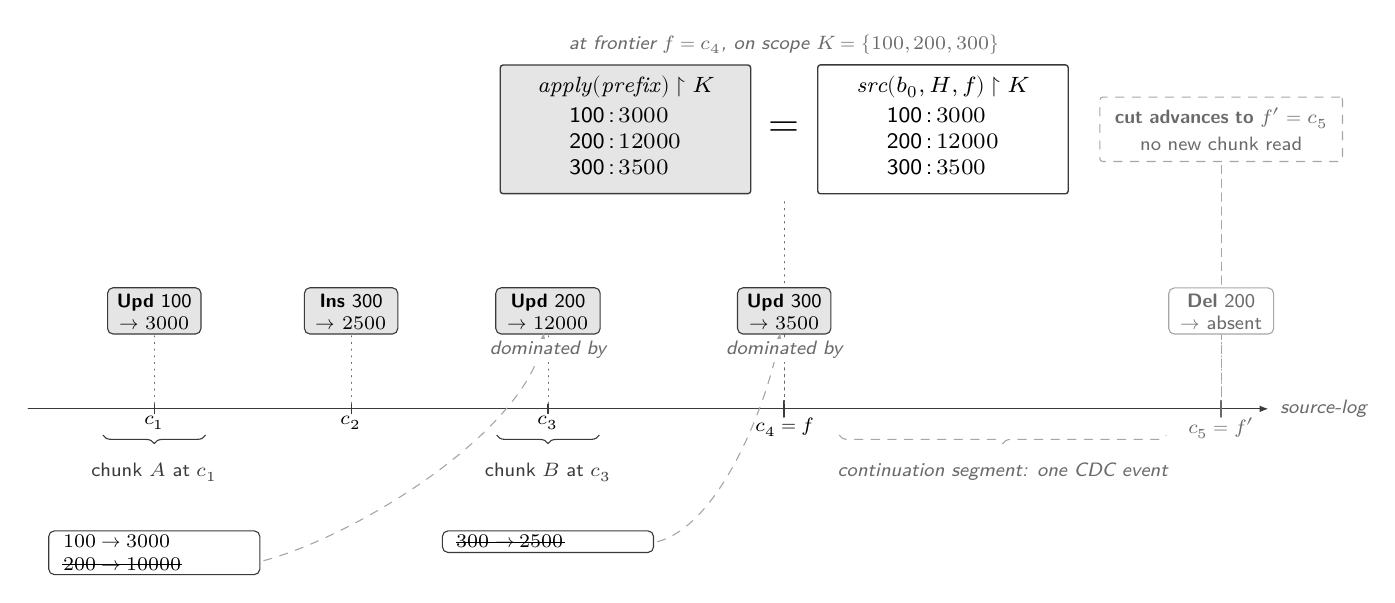
\begin{tikzpicture}[setA, x=1cm, y=1cm]

% ============================================================
% Coordinates (shared with Figure 3 -- running example).
% ============================================================
\def\xCa{1.50}
\def\xCb{4.00}
\def\xCc{6.50}
\def\xCd{9.50}
\def\xCe{15.05}                   % c_5 -- continuation-beat frontier
\def\axisY{0}
\def\writeY{0.85}
\def\brackY{-0.30}
\def\brackLabelY{-0.60}
\def\obsY{-1.55}

% ============================================================
% State equality at the top -- the "outcome at frontier" box.
% Two state cards side by side joined by "=".  The whole unit
% sits above the frontier coordinate c_4 so a vertical guide
% can rise from the axis into it.
% ============================================================
\def\eqY{3.55}                    % center y of the equality unit
\def\eqX{\xCd}                    % center x at the frontier

\node[font=\sffamily\Large, anchor=center] (eq) at (\eqX, \eqY) {$=$};

\node[blockFill, anchor=east, text width=29mm, align=center,
      left=4pt of eq.west, font=\sffamily\footnotesize]
  (lbox) {%
  \textbf{$\Apply(\CleanPrefix) \restrict K$}\\[1pt]
  \begin{tabular}{@{\ }r@{\,:\,}l@{\ }}
    100 & $3000$  \\
    200 & $12000$ \\
    300 & $3500$  \\
  \end{tabular}};

\node[block, anchor=west, text width=29mm, align=center,
      right=4pt of eq.east, font=\sffamily\footnotesize]
  (rbox) {%
  \textbf{$\Src(b_0, H, f) \restrict K$}\\[1pt]
  \begin{tabular}{@{\ }r@{\,:\,}l@{\ }}
    100 & $3000$  \\
    200 & $12000$ \\
    300 & $3500$  \\
  \end{tabular}};

% scope annotation above the equality unit
\node[sublabelDim, anchor=south] at ($(lbox.north -| eq) + (0,1.5pt)$)
  {at frontier $f = c_4$, on scope $K = \{100, 200, 300\}$};

% ============================================================
% Frontier guide -- dotted vertical from axis into the
% equality unit's south edge.
% ============================================================
\coordinate (eqSouth) at ($(eq |- lbox.south) + (0, -2pt)$);
\draw[guide, line width=0.5pt]
  (\xCd, \axisY) -- (eqSouth);

% ============================================================
% Source-log axis -- centered, with explicit endpoint padding.
% ============================================================
\draw[axisLine] (-0.10, \axisY) -- (15.65, \axisY);

\foreach \x/\lab in {\xCa/c_1, \xCb/c_2, \xCc/c_3} {
  \draw[axisTick] (\x, \axisY+0.06) -- (\x, \axisY-0.06);
  \node[anchor=north, font=\sffamily\scriptsize, inner sep=1pt]
    at (\x, \axisY-0.06) {$\lab$};
}
% Frontier tick c_4 is emphasized: heavier tick, bold label "c_4 = f".
\draw[axisTick, line width=0.8pt] (\xCd, \axisY+0.10) -- (\xCd, \axisY-0.10);
\node[anchor=north, font=\sffamily\scriptsize\bfseries, inner sep=1pt]
  at (\xCd, \axisY-0.08) {$c_4 = f$};

\node[sublabelDim, anchor=west, inner sep=0pt]
  at (15.80, \axisY) {source-log};

% ============================================================
% Source-log writes above the axis -- compact pills anchored
% at each commit coordinate.  Pills connect to the axis via a
% short downward leader.
% ============================================================
\foreach \x/\op/\key/\val/\tag in {%
  \xCa/Upd/100/$3000$/w_1,
  \xCb/Ins/300/$2500$/w_2,
  \xCc/Upd/200/$12000$/w_3,
  \xCd/Upd/300/$3500$/w_4%
} {
  \node[pillFill, anchor=south] (w-\tag) at (\x, \writeY+0.10) {%
    \strut\textbf{\op}~\key\\\,$\to$~\val\,};
  \draw[guide, line width=0.35pt] (\x, \axisY+0.07) -- (\x, \writeY+0.10);
}

% ============================================================
% Chunk-read brackets below the axis.
% ============================================================
% --- Chunk A at c1: observes 100 (kept) and 200 (becomes stale)
\draw[braceMirror] (\xCa-0.65, \brackY) -- (\xCa+0.65, \brackY);
\node[sublabel, anchor=north] (chAlab) at (\xCa, \brackLabelY)
  {chunk $A$ at $c_1$};

\node[pill, anchor=north, text width=24mm, align=left, inner xsep=4pt]
  (chAobs) at (\xCa, \obsY) {%
  \,$100 \to 3000$\\
  \,\sout{$200 \to 10000$}};

% --- Chunk B at c3: observes 300 (becomes stale)
\draw[braceMirror] (\xCc-0.65, \brackY) -- (\xCc+0.65, \brackY);
\node[sublabel, anchor=north] (chBlab) at (\xCc, \brackLabelY)
  {chunk $B$ at $c_3$};

\node[pill, anchor=north, text width=24mm, align=left, inner xsep=4pt]
  (chBobs) at (\xCc, \obsY) {%
  \,\sout{$300 \to 2500$}};

% ============================================================
% "Dominated by" leaders -- thin gray curves connecting each
% stale observation row to the source-log write that supersedes
% it.  These visually animate the strikethrough.
% ============================================================
% chunk-A row "200 -> 10000" is dominated by w_3 (Update 200 -> 12000)
\draw[weakFlow, rounded corners=2pt]
  ($(chAobs.east) + (0.05, -0.10)$)
  to[out=15, in=-100, looseness=0.7]
  ($(w-w_3.south) + (-0.05, 0.02)$);
% chunk-B row "300 -> 2500" is dominated by w_4 (Update 300 -> 3500)
\draw[weakFlow, rounded corners=2pt]
  ($(chBobs.east) + (0.05, 0)$)
  to[out=15, in=-100, looseness=0.7]
  ($(w-w_4.south) + (-0.05, 0.02)$);

% Labels on both leaders: "dominated by" -- placed just below each
% dominator write so they hug the dominator, not the axis.
\node[font=\sffamily\scriptsize\itshape, text=gMid, anchor=north,
      inner sep=1pt, fill=white]
  at ($(w-w_3.south) + (0, -0.06)$) {dominated by};
\node[font=\sffamily\scriptsize\itshape, text=gMid, anchor=north,
      inner sep=1pt, fill=white]
  at ($(w-w_4.south) + (0, -0.06)$) {dominated by};

% ============================================================
% Continuation beat -- advancing the cut to a later frontier
% c_5.  Drawn in a lighter register (dashed, gLight / gMid) to
% mark the continuation phase, distinct from the solid
% bootstrap depiction of the cut at c_4.
% ============================================================

% c_5 frontier guide -- dashed light, axis up into the c_5 card
% (the lighter parallel of the dotted c_4 frontier guide).
\draw[gLight, line width=0.4pt, densely dashed]
  (\xCe, \axisY) -- (\xCe, \eqY-0.45);

% c_5 source-log write pill -- dimmed (continuation phase).
\node[pill, draw=gLight, text=gMid, anchor=south] (w-w5)
  at (\xCe, \writeY+0.10) {\strut\textbf{Del}~200\\\,$\to$~absent\,};
\draw[guide, gLight, line width=0.35pt]
  (\xCe, \axisY+0.07) -- (\xCe, \writeY+0.10);

% c_5 tick -- emphasized like c_4 but dimmed; label "c_5 = f'".
\draw[axisTick, gMid, line width=0.8pt]
  (\xCe, \axisY+0.10) -- (\xCe, \axisY-0.10);
\node[anchor=north, font=\sffamily\scriptsize\bfseries, text=gMid,
      inner sep=1pt] at (\xCe, \axisY-0.08) {$c_5 = f'$};

% Continuation-segment bracket -- the c_4-to-c_5 source-log
% interval, below the axis in the lighter dashed register
% (parallel to the chunk-read brackets).
\draw[braceMirror, draw=gLight, dashed]
  (\xCd+0.70, \brackY) -- (\xCe-0.70, \brackY);
\node[sublabelDim, anchor=north]
  at ($(\xCd, \brackLabelY)!0.5!(\xCe, \brackLabelY)$)
  {continuation segment: one CDC event};

% c_5 advanced-cut card -- the lighter parallel of the c_4
% equality unit: the same cut, advanced to the later frontier.
\node[blockGhost, anchor=center, text width=28mm, align=center,
      font=\sffamily\scriptsize] (c5card) at (\xCe, \eqY) {%
  \textbf{cut advances to $f' = c_5$}\\[1.5pt]
  no new chunk read};

\end{tikzpicture}

\caption{Two chunk reads at different source-log coordinates assemble
into a replay whose state at frontier $f = c_4$ equals the source on
scope $K = \{100, 200, 300\}$. Stale observations (strikethrough) are
dominated by later source-log writes. No single physical read gathers
every key in scope, so the cut is virtual rather than physical.
That is the bootstrap cut at $c_4$. The lighter elements to the right
show the continuation of
Section~\ref{continuation-beat-advancing-the-cut}: one further
source-log event ($c_5$, a delete of account 200) is appended as the
continuation segment for the half-open interval $(c_4, c_5]$. It begins
strictly after the frontier $c_4$ and requires no additional chunk read. This advances
the same cut to the later frontier $f' = c_5$.}
\label{fig:running-example-timeline}

\end{figure*}

\subsection{What ``Snapshot-Equivalent'' Means
Here}\label{what-snapshot-equivalent-means-here}

There is no moment in this story when DBLog read the entire table at one
source-log position. Chunk A saw account 100 and account 200 at
$c_1$; chunk B saw account 300 at $c_3$. Because the two reads
happened at different points in the source database's commit order,
DBLog must reconcile them through the source log rather than read them
as one instantaneous observation.

What DBLog \emph{does} have is enough source-log evidence around each
chunk read to know which observations are still authoritative at the
chosen frontier and which have been superseded. That is the content of
the assembled replay sequence above: a deterministic mix of chunk-read
refreshes and CDC events that, taken together, have the same per-key
replay outcome as the source state at $f$ on the scope $K$.

The phrase ``snapshot-equivalent replay certificate without requiring
a single physical snapshot read'' is exactly this: the replay outcome
equals the
source state at $f$ restricted to $K$.

\subsection{What This Example Does Not
Show}\label{what-this-example-does-not-show}

The example is small on purpose. Several things it does \emph{not}
claim, and that the rest of the paper handles:

\begin{itemize}
\tightlist
\item
  \textbf{It is not a physical cut.} DBLog never performed a single read
  covering all of \{100, 200, 300\}: chunk A read accounts 100 and 200 at
  $c_1$, and chunk B read account 300 at $c_3$. The equivalence is
  \emph{extensional}: outcomes match at $f$ on $K$, not that DBLog secretly
  took a snapshot.
\item
  \textbf{It is not a whole-table claim.} The example claims only the
  three accounts in K. Other accounts in the source table are not
  addressed by this example. Whole-table correctness is a derived
  specialization handled later in the paper, with extra conditions
  attached.
\item
  \textbf{It is not a sink-state claim.} What we have shown is the
  assembled replay sequence. Whether a sink that consumes
  this sequence converges to the same per-account state is an additional
  contract on the consumer: idempotency, ordering, and fencing. The
  example does not engage that contract. The paper's later sections name
  the sink-state question explicitly and treat it as out of the
  headline.
\end{itemize}

\subsection{What Coordination DBLog Still
Needs}\label{what-coordination-dblog-still-needs}

Avoiding a physical snapshot read does not mean working without coordination.
The example silently relied on several pieces of source-side discipline
that the paper makes explicit later:

\begin{itemize}
\tightlist
\item
  A \textbf{source-log ordering} that is monotone and well-defined
  enough to compare the chunk-read coordinate of chunk A
  ($c_1$) to the CDC event for account 200 at
  $c_3$ and conclude that $c_3$ is later.
  Without a comparable ordering on commit positions, the ``later wins''
  rule cannot be applied.
\item
  \textbf{Chunk-read watermarks} placed in the source log around each
  chunk read, so DBLog can locate chunk A's read in source-log order
  --- placing its observation of account 200 before the $c_3$ event
  for account 200, and so recognizing that event as strictly newer.
  The example treats the chunk-read coordinate as known; the
  source-side mechanism that makes it known is the watermark bracket,
  made precise in the next section.
\item
  \textbf{Source-log retention}: the source log must still carry
  $c_1$ through $c_4$ when DBLog assembles the
  replay. If the log had truncated $c_1$ before chunk A was
  reconciled, the assembled replay would have a gap and DBLog would not
  be able to claim the scope $K$ up to $f$.
\item
  \textbf{Chunk-read consistency}: chunk A's two rows must both reflect
  the source at the single coordinate $c_1$. The watermark bracket
  locates the read in source-log order but does not by itself
  establish that single-coordinate attribution; a consistent
  statement-level read, or per-row coordinate evidence, is what the
  deployment must supply.
  Section~\ref{watermarks-and-chunk-read-coordinates} makes this
  obligation precise.
\end{itemize}

These are concrete operational obligations on the deployment, not
features DBLog removes. They reappear in the formal model as explicit
predicates and assumptions, and again in the closing sections as
deployment obligations and external observation assumptions.

\subsection{What Comes Next}\label{what-comes-next}

The next section names the operational vocabulary used above precisely:
chunk plan, watermarks, refresh events, ordinary CDC events, raw replay,
normalized clean prefix, stale-refresh dominance at replay time, clean
prefix, frontier, scope. The section after that states what DBLog is,
what it is not, and which failure modes matter; the formal sections then
lift those names into definitions, and the per-account map produced by
the seven-item replay sequence becomes the object the central theorem
equates with the source state at the chosen frontier restricted to the
chosen scope. By the time we reach the theorem statement, every move in
this section will have a named formal counterpart.

The paper later proves the general theorems this example is meant to
illustrate. Playing the seven-item replay sequence produces the same
per-account map as the source state at the frontier $f = c_4$ restricted
to $K$; appending the eighth item then advances that cut to the later
frontier $f' = c_5$.

\section{The DBLog Mechanism}\label{the-dblog-mechanism}

The running example used two chunks and four source-log events. This
section abstracts from that example to the DBLog mechanism itself. The
goal is not yet to prove the theorem; the goal is to give names to the
operational pieces that the theorem later constrains.
Figure~\ref{fig:dblog-mechanism} walks the same running example through
the mechanism's coordinate axis, source-log events, refresh windows,
and the merged raw-replay matrix.

\begin{figure*}[t]
  \input{figures/fig03_dblog_mechanism/fig03.tex}
\end{figure*}

\subsection{Chunks and Scope}\label{chunks-and-scope}

DBLog begins with a \textbf{scope}: the set of primary keys for which
the backfill will make a claim. In the example, the scope was the three
account ids \{100, 200, 300\}. In a larger deployment the scope might be
a table, a shard, a tenant, or a selected key range.

The scope is partitioned into \textbf{chunks}. Each key in the claimed
scope belongs to exactly one responsible chunk in the model used by this
paper. That strict ownership rule is not incidental. If two chunks both
own the same key, or if a key in the claimed scope belongs to no chunk,
then the replay no longer has a single disciplined source for that key's
refresh evidence. Overlap and retry can be modeled, but not by
pretending strict ownership still holds; the paper treats richer
overlap/retry schemes as future extensions unless their normalization is
made explicit.

The model also abstracts from how the finite chunk plan is discovered.
A deployment must still know when the chunk loop has reached the
intended end of the claimed key scope. For a whole-table run, a common
way to establish that fact is to record the table's maximum primary key,
or an equivalent end-of-table observation, with enough source-side
context to know which table population the bound refers to. For a
selected range, shard, tenant, or other scoped run, the analogous
obligation is an end-of-scope witness for that chosen scope. This is a
Deployment obligation; faithfulness of the primary-key ordering and of
the source-side observation that supplies the bound remains an External
observation assumption.

\subsection{Watermarks and Chunk-Read
Coordinates}\label{watermarks-and-chunk-read-coordinates}

A chunk read has to be located in source-log time: to merge a chunk's
rows with the live CDC stream, DBLog must know which source-log events
precede the chunk's observations and which supersede them. The mechanism
that establishes this is the \textbf{watermark}. Just before it begins a
chunk read, DBLog writes a marker row --- a \emph{low watermark} --- into
a dedicated watermark table in the source; when the chunk scan finishes,
it writes a second marker, the \emph{high watermark}. Both are ordinary
source writes, so both surface in the source change log at definite
coordinates, and the chunk \texttt{SELECT} ran between them. These
watermark writes mean the baseline mechanism needs write access to the
source database; a deployment that cannot write to the source would
need another way to locate its chunk reads in the log.

The watermark pair establishes \emph{provenance}: it brackets the chunk
read in source-log order, fixing which committed source events precede
the read and which follow it. The model then attributes the whole chunk
read to a single \emph{chunk-read coordinate} --- the running example's
``chunk A read at $c_1$'' --- and treats every row image the chunk
returned as faithful to the source at that coordinate. That
single-coordinate attribution is a \emph{stronger} fact than the
watermark bracket alone supplies. A multi-row chunk \texttt{SELECT} is
not instantaneous, so the bracket locates the read but does not by
itself prove that every returned row image reflects the source at one
shared coordinate. The attribution is sound only when the deployment
also supplies one of two things: chunk-read semantics that make the
returned rows a consistent read at a single source coordinate --- for
instance a statement-level snapshot or repeatable-read scan --- or
per-row coordinate evidence pinning each returned image to the
coordinate at which it held. The shorthand ``chunk A read at $c_1$''
therefore stands for both facts together: chunk A's watermarks bracket
$c_1$, \emph{and} chunk A's row images are faithful to the source at
$c_1$.

In the original DBLog mechanism the watermark pair does more than locate
the read: the interval between the low and the high watermark is also the
window over which stale chunk rows are suppressed --- a chunk row is
discarded when the source log shows a write for the same key inside that
window. This paper's model abstracts that windowed interleaving into two
simpler pieces: a single chunk-read coordinate at which each returned row
image is faithful, and a frontier-wide \emph{latest-event-wins} replay
(\S\ref{refresh-events-and-ordinary-cdc-events}). The two views reach the
same per-key state, by the window-suppression equivalence of
\S\ref{raw-replay-and-normalized-clean-prefix}. A write committed inside
the watermark window is
itself an ordinary CDC event the replay carries, and latest-event-wins
lets it override the chunk row exactly as in-window suppression would; a
write after the high watermark is carried the same way. So ``suppressed
inside the window'' and ``overridden later, at the frontier'' are the
same fact. The low and high watermarks are kept in the formal run only as
the operational provenance of the chunk-read coordinate; they carry no
separate state-equality obligation of their own beyond the
chunk-read-coordinate provenance and row-image honesty obligations
\S\ref{wellformed-runs} makes explicit. The watermark pair is
therefore the deployment's \emph{means} of establishing that
coordinate, not a formal object the theorem itself consults.

Both facts are deployment obligations, not properties DBLog establishes
for free: a source log that exposes an ordering and is retained long
enough for DBLog to compare chunk rows against later CDC events, and the
single-coordinate row-image faithfulness just described.
\S\ref{wellformed-runs} carries them as wellformed-run obligations, with
the row-image fact appearing as the ``Refresh honesty'' obligation.

DBLog avoids a single physical snapshot read; it does not avoid source-log
coordination.

\subsection{Refresh Events and Ordinary CDC
Events}\label{refresh-events-and-ordinary-cdc-events}

DBLog turns each chunk-read row into a \textbf{refresh event}. A refresh
says: ``at this chunk-read coordinate, key $k$ was observed with this
value,'' or ``key $k$ was observed absent.'' A source-log write becomes an
ordinary CDC event: insert, update, or delete at its source-log
coordinate.

Both kinds of event enter one replay vocabulary. Ordinary CDC events
carry committed source writes. Refresh events carry row observations
from chunk reads. Applying a replay means walking the event sequence
left to right and updating the per-key state; later events for the same
key win. That latest-event-wins behavior is what made Bob's $c_3$ update
override chunk A's older refresh in the example.

\subsection{Raw Replay and Normalized Clean
Prefix}\label{raw-replay-and-normalized-clean-prefix}

The replay evidence DBLog assembles is one finite sequence, the
\emph{clean prefix}, and it comes in two forms. This subsection defines
both. The theorems in this paper are stated about the \emph{raw} form;
the \emph{normalized} form is an optional, $\Apply$-equivalent
presentation.

The \textbf{raw replay} is the evidence-preserving sequence: it may
include a refresh even if a later CDC event for the same key dominates
it. Raw replay is useful operationally because it shows exactly what
DBLog observed.

The \textbf{normalized clean prefix} is an optional, $\Apply$-equivalent
view: the formal development takes the raw clean prefix as its proof object,
and normalization is a presentation that makes stale-refresh suppression
explicit. It may suppress refresh events that are dominated by newer
source-log evidence, provided suppressing them does not change the final
$\Apply$ state. In the example, Bob's chunk-A refresh was
dominated by Bob's later c3 update; Carol's chunk-B refresh was
dominated by Carol's later c4 update. Carrying or suppressing those
dominated refreshes gives the same final per-key state. The proof-facing
bridge is state equivalence on the claimed scope: suppressing only
same-key dominated refreshes preserves $\Apply$ for every claimed
key.

\smallskip
\noindent\textbf{Window-suppression equivalence.} \emph{Retaining or
suppressing a same-key refresh that a later source event dominates
leaves $\Apply$ unchanged on every claimed key.} This is the fact that
lets the raw and normalized clean prefixes be used interchangeably, and
it is also why original DBLog's in-window suppression and this paper's
frontier-wide latest-event-wins reach the same per-key state: a refresh
overridden inside the watermark window and a refresh overridden later at
the frontier are dominated the same way, so $\Apply$ does not
distinguish them.
Section~\ref{source-side-virtual-cut-soundness-layer-2} uses this
equivalence to state the Layer~2 theorem about the raw clean prefix
while leaving normalization an optional presentation.

The theorem later relies on both sides of this story:

\begin{itemize}\tightlist
\item no required CDC event is missing;
\item no stale refresh is allowed to resurrect an older value past a
  newer event;
\item suppressing a refresh is justified only when newer source-log
  evidence dominates it for the same key.
\end{itemize}

\subsection{Frontier and Clean Prefix}\label{frontier-and-clean-prefix}

The \textbf{frontier} is the source-log coordinate at which a cut is
claimed (concretely, a MySQL executed global-transaction-identifier
(GTID) set, a PostgreSQL log sequence number (LSN), or a
CockroachDB resolved timestamp). A certificate does not merely claim ``some eventual state''; it
claims equality at a particular frontier. The clean prefix contains the
replay evidence needed through that frontier for the claimed scope.

Operationally, a DBLog certificate is useful only when the operator can
say:

\begin{quote}
\itshape
for this scope $K$ and frontier $f$, here is the finite replay prefix
whose application equals the source state at $f$ on $K$.
\end{quote}

The rest of the paper makes that sentence precise. Section~5 defines the
source and replay models. Section~6 names the equality as a virtual cut.
Section~7 proves the source-side theorem for wellformed runs. Sections~8
and~9 move from runs to accepted certificates.

The clean prefix is finite but not necessarily small. It carries a
refresh for each key in the claimed scope and every in-scope CDC event
through the frontier, so it scales with the scope and the change
volume over the certified interval --- for a large table backfilled
over a busy window it is a correspondingly large object. The
normalized clean prefix trims refreshes that newer evidence dominates;
the raw form, on which the theorems are stated, does not.

\subsection{After the Chunk Loop: Advancing the
Frontier}\label{after-the-chunk-loop}

The backfill chunk loop is finite: it runs until the claimed key scope
is covered, and then it closes. But the frontier of a virtual cut is not
the end of DBLog's story. Once the chunk loop has established a virtual
cut at a frontier $f$, DBLog continues as ordinary change-data-capture,
consuming source-log events as the source commits them. The source-side
story does not need a fresh chunk read for every later frontier. If the
source log faithfully supplies the change data the source committed
after $f$ and through a later frontier $f'$, appending that segment to
the clean prefix advances the replay-equivalence claim from $f$ to $f'$.

This is the operational reading of the continuation result proved in
Section~\ref{source-side-continuation-and-restriction}: the backfill
bootstraps the first virtual cut, and faithful CDC continuation advances
it. The chunk reads are the hard part, and they happen once; advancing
the established cut to a later frontier is then appending faithful
source-log change data. Carrying the cut forward leans on the same
source-side discipline the chunk loop already needed --- a source-log
ordering, and retention of the events between $f$ and $f'$ --- and
Section~\ref{source-side-continuation-and-restriction} states the result
and its premises precisely.

\smallskip
\noindent\textbf{Practitioner takeaway.} \emph{DBLog's mechanism is a
small fixed vocabulary: a key scope split into chunks, watermark-bracketed
chunk reads attributed to a chunk-read coordinate, refresh events and
ordinary CDC events merged into one clean prefix, and a frontier at
which the cut is claimed. None of it is free of coordination --- a
deployment owes a source log that is ordered and retained, chunk reads
whose row images are faithful to their coordinate, and a finite chunk
partition of the scope. Those obligations, not the watermark trick, are
what a real backfill must get right.}

\section{What DBLog Is, What It Is Not, and Its
Limitations}\label{what-dblog-is-what-it-is-not-and-its-limitations}

DBLog is a source-side CDC-plus-chunk-read evidence protocol: live
backfill establishes an initial virtual cut, and faithful CDC
continuation can advance that cut to later source frontiers. It is a way
to synthesize a replay-equivalent stand-in for a snapshot on a chosen
scope at a chosen frontier, and to carry that stand-in forward as the
source frontier moves. It is not a loophole around coordination,
observation faithfulness, or destination semantics. This section states
those boundaries before the formal sections begin.

\subsection{What DBLog Is}\label{what-dblog-is}

DBLog is a source-side evidence protocol. It combines:

\begin{itemize}\tightlist
\item a claimed key scope;
\item a certified frontier in source-log order;
\item chunk reads whose observations become refresh events;
\item ordinary CDC events from the source log;
\item source-log and chunk-read evidence sufficient to justify the
  clean prefix;
\item a finite replay prefix whose $\Apply$ state can be compared with
  the source;
\item a source-side continuation principle: an established virtual cut
  advances to a later source frontier by appending the faithful change
  data the source committed in between.
\end{itemize}

The paper's positive claim is extensional: replaying the clean prefix
reaches the same state as the source at the frontier, restricted to the
claimed scope. The certificate does not make the source pause, and the
theorem does not need a physical snapshot read.

\subsection{What DBLog Is Not}\label{what-dblog-is-not}

DBLog is not coordination-free. It needs source-log ordering, retained
CDC events, chunk-read coordinates, frontier discipline, and evidence
tying those observations to the source. These are Deployment obligations
or External observation assumptions, not details the theorem erases.

DBLog is not exactly-once delivery. The theorem is about the state
reached by replay, not about how many times a downstream transport
delivers an event.

DBLog is not whole-table correctness by default. The core theorem is
scoped. Whole-table equality appears later as a derived specialization
and only under explicit anchor-domain and no-unclaimed-replay-key side
conditions.

DBLog is not sink-state correctness. A destination can receive a
certified stream without having applied it, applied it in the intended
order, or reached the corresponding state.
Section~\ref{sink-state-convergence-non-claim} records this as a
Non-claim.

DBLog is not continuous destination replication. The source-side
continuation result
(Section~\ref{source-side-continuation-and-restriction}) advances a
virtual cut to later source frontiers; it does not show that a sink has
applied the replay, applied it once, or reached the corresponding state.

DBLog is not a claim that a single physical source-read timestamp
existed for all chunk rows. A virtual cut is an equality of outcomes,
not a hidden physical cut.

DBLog is not a product-by-name theorem. Debezium, Apache Flink CDC, and
source engines such as MySQL, PostgreSQL, and MariaDB are relevant
deployment and related-work contexts. This paper does not claim that any
named system satisfies the theorem without checking the paper's
assumptions against that system.

\subsection{Failure Modes the Certificate Story Must
Expose}\label{failure-modes-the-certificate-story-must-expose}

Table~\ref{tab:failure-modes} is intentionally operational. It says
what can go wrong, which part of the evidence story is responsible for
catching it, and how the paper classifies the obligation.

\begin{table*}[t]
\caption{Failure modes the certificate story must expose, with the
evidence or assumption boundary each touches and its status.}
\label{tab:failure-modes}
\centering\small
\begin{tabularx}{\textwidth}{@{}p{1.55in}YYY@{}}
\toprule
\textbf{Failure mode} & \textbf{What goes wrong} &
\textbf{Evidence or assumption boundary} & \textbf{Status}\\
\midrule
Missing CDC event &
  A source write in the claimed interval is absent from the replay
  evidence. &
  Source-log retention and CDC coverage through the certified
  frontier. &
  Deployment obligation / External observation assumption\\
Missing continuation segment &
  A later frontier is claimed without the faithful source-log change
  data the source committed between the certified frontier and that
  later frontier. &
  Source-log retention for the continuation interval and faithful CDC
  coverage. &
  Deployment obligation / External observation assumption\\
Bad watermark or coordinate &
  A chunk row is treated as if it was read at the wrong source-log
  position. &
  Watermark or coordinate faithfulness for the chunk read. &
  Deployment obligation / External observation assumption\\
Stale refresh survives &
  An older chunk-read value overrides a newer source-log event for
  the same key. &
  Clean-prefix dominance and latest-event ordering. &
  Conditional\\
Wrong frontier &
  The replay is certified against a frontier different from the
  source interval it actually covers. &
  Frontier consistency in the certificate and evidence. &
  Conditional\\
Scope ownership mismatch &
  A claimed key is not owned by exactly one responsible chunk, or the
  claimed scope does not match the chunk plan. &
  Chunk ownership and claim-scope checks. &
  Conditional\\
Incomplete chunk-plan termination &
  The chunk loop stops before the intended end of the key range, so a
  key in the intended operational scope may be absent from the finite
  plan; for a whole-table claim, the anchor domain is not shown to be
  covered. &
  Chunk-plan construction, maximum-key or end-of-scope evidence,
  primary-key ordering, and whole-table claim-scope coverage. &
  Deployment obligation / External observation assumption\\
Whole-table replay-key mismatch &
  The whole-table specialization is requested while replay evidence
  materializes keys outside the claim scope. &
  Layer 4 no-unclaimed-replay-key side condition; not part of scoped
  virtual-cut equality. &
  Conditional\\
Unfaithful observation &
  The connector, source log, primary-key interpretation, or
  chunk-read result is not faithful to the real database. &
  Not internally provable from the certificate alone. &
  External observation assumption\\
\bottomrule
\end{tabularx}
\end{table*}

The operational rows above, for the initial certificate, are the kind a
certificate checker can make visible against the evidence bundle, under
the source-side model and, for whole-table lifting, under the extra
Layer 4 side condition. The continuation row is the exception: advancing
a cut to a later frontier reuses the same evidence-boundary discipline,
but a concrete checker for extended certificates is Future work. The
final row is the trust boundary: the paper assumes faithful source
observation when it turns accepted evidence into a theorem about the
mathematical source history. Acceptance alone is not the theorem.

\subsection{The Main Limitation to Keep in
Mind}\label{the-main-limitation-to-keep-in-mind}

The strongest current statement in the paper is still source-side. It
says that accepted evidence, under faithful source observation and the
checker substrate obligations, yields a certified virtual cut. It does
not say that a concrete parser is correct, that a connector never
misreports the source, that a named product implements every assumption,
or that a sink has applied the certified replay to state. Those are all
meaningful engineering questions. This paper's contribution is to make
clear which ones are inside the theorem and which ones remain
obligations or future work.

\smallskip
\noindent\textbf{Practitioner takeaway.} \emph{Read DBLog as a
source-side evidence protocol with sharp edges: it is a replay-equivalent
stand-in for a snapshot on a chosen scope and frontier, advanceable to
later frontiers --- and it is none of the things the boundaries above
rule out, including exactly-once delivery, whole-table correctness by
default, sink-state convergence, and product-by-name transfer. The
failure-mode table is the operational checklist; the standing trust
boundary is faithful source observation, which no certificate settles
from the inside.}

\section{Formal Model \mbox{(Layer 0 and Layer 1)}}\label{formal-model-layer-0-and-layer-1}

The formal model begins with two deliberately small layers. Layer 0
defines the source and replay vocabulary: source histories, source state
at a frontier, replay events, replay application, and restriction to a
key scope. Layer 1 defines abstract DBLog runs: chunks, watermarks,
chunk reads, ordinary CDC observations, clean prefixes, and the
wellformedness obligations that make the source-side theorem true.

Neither layer mentions certificates, verifiers, destination ACKs, or
whole-table side conditions. That separation matters. Layer 2 proves a
theorem about wellformed runs. Layer 3 later explains when an accepted
certificate witnesses such a run.

Table~\ref{tab:notation} fixes the symbols the formal sections use. A
predicate (short sans-serif tag like $\WF$, $\FSO$, $\Mat$, $\Coh$,
$\VC$, $\WTS$) is a relation that holds or fails on its arguments; an
accessor function (italic word like $\Apply$, $\Src$, $\Scope$,
$\Frontier$, $\CleanPrefix$) returns a value.

\begin{table*}[t]
\caption{Notation used in the formal model and theorem statements.
Predicates are rendered in sans-serif; accessor functions in italic.}
\label{tab:notation}
\centering\small
\begin{tabularx}{\textwidth}{@{}l@{\hskip 1em}l@{\hskip 1em}Y@{}}
\toprule
\textbf{Symbol} & \textbf{Kind} & \textbf{Read as}\\
\midrule
$b_0$, $H$, $f$ & variables &
  base state, source history, frontier coordinate.\\
$b$, $f'$ & variables &
  whole-table anchor source coordinate ($b \le f$); later source
  frontier (continuation target; $f \le f'$).\\
$R$, $C$, $E$ & variables &
  abstract DBLog run, certificate, evidence bundle.\\
$\sigma$, $\delta$, $K$ & variables &
  replay sequence, continuation segment (CDC replay-event list),
  key scope.\\
$\Src(b_0,H,f)$ & accessor & source state at frontier $f$.\\
$\Apply(\sigma)$ & accessor & replay-apply of sequence $\sigma$.\\
$\Scope(\cdot)$ & accessor & claimed key scope (of run or certificate).\\
$\Frontier(\cdot)$ & accessor & chosen source-log frontier.\\
$\CleanPrefix(\cdot)$ & accessor & clean replay prefix.\\
$m \restrict K$ & operator & state $m$ restricted to keys in $K$.\\
$\Verify(C,E)$ & accessor &
  verifier result, one of $\Accept$, $\Reject$, $\Unsupported$.\\
$\RawObs$ & variable &
  raw source-observation carrier (External observation assumption).\\
$\AnchorDomain(H,b)$ & accessor & keys present at the anchor boundary $b$.\\
$\TouchedBetween(H,b,f)$ & accessor & keys with source events in $(b,f]$.\\
$\TableScopeBetween(H,b,f)$ & accessor & union of the two above.\\
$\ReplayKeys(\sigma)$ & accessor & keys written by replay sequence $\sigma$.\\
$\Chunks(R)$ & accessor & run's chunk plan.\\
$\SourceHistory(R)$ & accessor & source history the run is about.\\
$\CdcEvents(R)$ & accessor & CDC events the run consumed.\\
\midrule
$\WF(b_0,R,H)$ & predicate &
  wellformed DBLog run (Layer 1).\\
$\VCS(\sigma,K,f,H)$ & predicate &
  state-level virtual cut (Section~\ref{virtual-cuts}); the base state
  $b_0$ is implicit in this four-argument shorthand and made explicit
  in the unfolded form in Section~\ref{virtual-cuts}.\\
$\VC(C,H)$ & predicate &
  certificate-side virtual cut.\\
$\ContSeg(H,K,f,f',\delta)$ & predicate &
  $\delta$ is the continuation segment for $(f,f']$ on $K$
  (Section~\ref{source-side-continuation-and-restriction}).\\
$\Mat(C,E,R)$ & predicate &
  $(C,E)$ materializes abstract run $R$.\\
$\Coh(C,E,R)$ & predicate &
  $(C,E)$ is coherent with run $R$ (Section~\ref{certificate-run-coherence}).\\
$\FSO(E,b_0,H,\RawObs)$ & assumption &
  faithful source observation.\\
$\WTS(C,H,b)$ & predicate &
  whole-table claim scope (Layer 4).\\
\bottomrule
\end{tabularx}
\end{table*}

\subsection{Source Histories and
Frontiers}\label{source-histories-and-frontiers}

A source database is modeled as a base state $b_0$ together with a
finite history $H$ of committed source events. A source event is
one of
\[
  \mathsf{Insert}\,k\,v,\qquad
  \mathsf{Update}\,k\,v,\qquad
  \mathsf{Delete}\,k.
\]
Each event carries a source coordinate: a commit position, log sequence
number, monotone source-side timestamp, or equivalent order-bearing
token. We write $c \le c'$ when
coordinate $c$ is no later than $c'$. A
source history is wellformed when its events are ordered by that
coordinate, the base coordinate sits before every event, and
same-coordinate events have a deterministic source-position order inside
the history.

The source state at a frontier is written $\Src(b_0,H,f)$.
For each key $k$, this state looks for the latest source event
for $k$ at or before frontier $f$. An insert or update
makes the key present with the written value; a delete makes it absent;
no event leaves the key at its base state $b_0(k)$.

The coordinate convention is inclusive. A chunk read recorded at
coordinate $c$ observes $\Src(b_0,H,c)$, including
source events at coordinate $c$. The convention is not an arbitrary
tie-break: a chunk read is \emph{attributed} to the latest coordinate
whose committed effects its row images already reflect.
\S\ref{watermarks-and-chunk-read-coordinates} sets out what a deployment
must supply for that attribution to be sound --- the watermark bracket
locating the read, together with the chunk-read semantics or per-row
coordinate evidence that make the returned row images faithful to one
coordinate. Canonical replay therefore
places same-coordinate CDC evidence before the refresh that records the
post-$c$ chunk-read state. Later source-coordinate events still
appear after that refresh.

This is the source-side reference state that every virtual-cut theorem
compares against.

\subsection{Replay Events and Apply}\label{replay-events-and-apply}

DBLog does not replay source events alone. It replays two kinds of
replay event:
\[
  \begin{array}{ll}
    \mathsf{Cdc}\,c\,e & \text{source-log event $e$ at coord.\ $c$,}\\
    \mathsf{Refresh}\,k\,m\,c & \text{chunk-read of $k$ at coord.\ $c$.}
  \end{array}
\]
In a refresh, $m = \mathsf{Some}\,v$ means the chunk read observed
value~$v$; $m = \None$ means the chunk read observed row
absence. Absence is a state fact, not an exception: replaying a refresh
with $\None$ deletes the key from the replay state.

The replay function is $\Apply(\sigma)$, where $\sigma$ is a finite
replay sequence. $\Apply$ walks the sequence from left to right,
updating a per-key map. Later events
for the same key win. $\Apply$ starts from the all-absent per-key
map: $\Apply([\,])(k) = \None$ for every key~$k$. Thus the running
example's later update for Bob overrides chunk A's older refresh, and
a later delete would override both an earlier refresh and an earlier
update.

State restriction is written $m \restrict K$ in prose formulas
below: it keeps only the entries whose keys lie in $K$, so
$(m \restrict K)(k) = m(k)$ when $k \in K$, and
$\None$ otherwise. The displayed formulas use the
$\restrict$ symbol throughout.

% Float declared upstream of \subsection{Wellformed Runs} so LaTeX can
% place Table 4 at the top of an earlier page than where its body-text
% intro paragraph naturally sits.  Source position pins the earliest
% page a top-float can land on --- floats only move forward.  Declaring
% the float near its intro paragraph (in \S5.5 source) pinned earliest
% top-placement at page 14, leaving column 2 of that page short below
% the table; an upstream declaration (here, before \S5.3) lets LaTeX
% place the float on page 13.  Rendering order is unchanged --- the
% caption block stands on its own and \S5.5 still introduces it with
% ``Its clauses say:'' wherever the float lands.
\begin{table*}[t]
\caption{Wellformed-DBLog-run obligations: clauses of
$\WF(b_0,R,H)$ in reader-facing terms, with status.}
\label{tab:wellformed-obligations}
\centering\small
\begin{tabularx}{\textwidth}{@{}p{1.45in}Yp{1.8in}@{}}
\toprule
\textbf{Obligation} & \textbf{Meaning} & \textbf{Status}\\
\midrule
Source binding &
  $R$ is about source history $H$, and $H$ is wellformed. &
  Deployment obligation\\
Chunk partition &
  The chunks form a finite strict partition of $\Scope(R)$. &
  Deployment obligation\\
CDC coverage &
  Every relevant source event after the responsible chunk read and
  through the frontier is observed. &
  External observation assumption\\
CDC faithfulness &
  Observed CDC events are real source events, in the right order, with
  same-key same-coordinate multiplicity preserved. &
  External observation assumption\\
Chunk evidence &
  Chunk read coordinates are bracketed by watermarks, and chunk-read
  observations produce the corresponding value-or-absence refreshes for
  claimed keys. &
  Deployment obligation\\
Read-before-frontier &
  Every chunk read occurs no later than the run frontier. &
  Deployment obligation\\
Refresh honesty &
  A chunk-read value or absence matches
  $\Src(b_0,H,\text{read-coord.})$ for that key. &
  External observation assumption / Deployment obligation\\
\bottomrule
\end{tabularx}
\end{table*}

\subsection{Abstract DBLog Runs}\label{abstract-dblog-runs}

A DBLog run $R$ is held abstract. The model observes it only
through a small set of accessors:
\[
  \begin{aligned}
    \Scope(R)\quad             &\text{claimed key scope},\\
    \Frontier(R)\quad           &\text{chosen source frontier},\\
    \CleanPrefix(R)\quad        &\text{replay sequence of the run},\\
    \Chunks(R)\quad             &\text{run's chunk plan},\\
    \SourceHistory(R)           &\ \text{source history the run is about},\\
    \CdcEvents(R)               &\ \text{observed CDC events consumed.}
  \end{aligned}
\]
Each chunk has a domain of keys, a responsible-chunk relation from
keys to chunks, a lower and upper watermark, and a chunk-read
coordinate. The model uses a strict canonical partition: each key in
$\Scope(R)$ belongs to exactly one responsible chunk, and every
responsible chunk has a finite domain. The model also takes the chunk
plan itself to be finite --- the set of chunks is finite for every
run. This is a modeling assumption, not a proof-engineering detail: it
reflects that a real backfill runs a bounded chunk loop over a finite
plan.

That strict partition is not a claim that real systems never retry or
overlap chunk reads. It is the canonical run selected for the theorem.
Raw overlap/retry evidence must be normalized into such a canonical run,
or handled by a future extension.

\subsection{Clean Prefix}\label{clean-prefix}

The clean prefix of a run is the finite replay sequence produced from:

\begin{itemize}\tightlist
\item chunk-read refreshes for the responsible chunks;
\item observed CDC events for in-scope keys through the frontier;
\item the \emph{clean-prefix ordering}: events sorted by source
  coordinate, with a CDC event placed before a chunk refresh at a
  shared coordinate, and same-coordinate CDC events kept in
  source-log position order;
\item suppression, or harmless retention, of refreshes dominated by
  newer same-key source-log evidence.
\end{itemize}

The theorem does not rely on a mysterious ``good replay'' primitive. The
clean prefix is constrained by the run's chunk plan, CDC observations,
frontier, and scope. If a needed CDC event is missing, if a future event
is replayed, if a refresh appears without a responsible chunk
observation, or if same-coordinate CDC order is scrambled, the run is
not wellformed for the theorem.

The proof-facing bridge invariant is per-key: for each key in scope, the
latest replay event in the clean prefix is either the latest faithful
source event through the frontier, or it is a refresh whose value or
absence at its read coordinate remains unchanged until the frontier.
This is the invariant Layer 2 unfolds rather than assuming as a
primitive.

One mechanization-level premise rides along with this construction:
the canonical clean prefix enumerates each chunk domain in sorted key
order, so the run- and certificate-layer theorems assume a linear
order on the key type --- in practice the primary-key order a chunked
backfill already presupposes. The state-level continuation and
restriction theorems of
Section~\ref{source-side-continuation-and-restriction} carry no such
constraint.

\subsection{Wellformed Runs}\label{wellformed-runs}

We write $\WF(b_0,R,H)$ for the wellformed DBLog run predicate; it
packages the source-side obligations the proof needs. Its clauses
say, in reader-facing terms:

The split between Deployment obligation and External observation
assumption is intentional. The model can state what a wellformed run
must satisfy. It cannot prove, from inside the run, that an external
database connector reported every source event honestly or that a chunk
read was faithful to the real source.

Refresh honesty carries both labels because it bundles two facts: that
a returned row image reports the source value or absence faithfully is
an External observation assumption, while that the chunk-read semantics
pin those images to a single coordinate
(\S\ref{watermarks-and-chunk-read-coordinates}) is a Deployment
obligation.

The wellformed-run predicate carries one further conjunct, not listed
above: clean-prefix closure. It is \emph{definition-derived} --- it
holds for every run by the clean-prefix construction
(Section~\ref{clean-prefix}) --- so it is neither a deployment
obligation nor an external observation assumption, and no wellformed
run can fail it. The proof may use it; no deployment need establish it
separately.

The lower and upper watermarks introduced above are source-log
coordinates, not primary-key-range bounds. Accordingly, the Chunk
partition row is a statement about the finite canonical partition
consumed by the theorem; it is not a proof that a concrete
chunk-selection loop stopped in the right place, and Layer 1 contains no
maximum-key accessor or chunk-loop termination algorithm. A
maximum-primary-key query, an empty-next-chunk observation, a
predeclared range bound, or another end-of-scope witness may justify the
finite partition operationally. Supplying the resulting partition,
including evidence that the loop reached the intended end of the
claimed key scope, is a Deployment obligation; the theorem consumes the
partition, not the plan-construction algorithm.

\subsection{Layer 0 and Layer 1
Lemmas}\label{layer-0-and-layer-1-lemmas}

The source and replay model supplies the elementary facts used by the
main proof:

\begin{itemize}\tightlist
\item $\Apply$ is latest-event-wins per key.
\item Restricted states are equal exactly when they agree on every key
  in the scope.
\item $\Src$ is characterized by the latest source event at or before
  the frontier.
\item A replay-side $\mathsf{Cdc}$ event has the same per-key effect as
  its source event.
\item A refresh has the source-state value at its chunk-read coordinate
  when the chunk-read honesty premise holds.
\item The source state at a later frontier is the source state at an
  earlier frontier updated by exactly the source events strictly
  between them --- immediate from the preceding characterization, since
  the source events at or before $f'$ are those at or before $f$
  together with those in $(f,f']$. This interval characterization is
  what the continuation result of
  Section~\ref{source-side-continuation-and-restriction} builds on.
\end{itemize}

The run layer then contributes the bridge lemma:

\[
\begin{aligned}
  \WF(b_0,R,H) \,\Longrightarrow{}&
    \Apply(\CleanPrefix(R)) \restrict \Scope(R)\\
  &{}= \Src(b_0,H,\Frontier(R)) \restrict \Scope(R).
\end{aligned}
\]

That bridge is the Layer 2 theorem stated and explained in Section~7.
Section~6 first names the equality itself.

\smallskip
\noindent\textbf{Practitioner takeaway.} \emph{The objects in this
section are the paper's working vocabulary; the part a real deployment
must act on is the wellformed-run obligation table
(Table~\ref{tab:wellformed-obligations}) --- source-log retention and
binding, a finite chunk partition, watermark-bracketed chunk reads, and
CDC coverage and faithfulness. A backfill that meets those obligations is
exactly the kind of run the soundness theorems in the following sections
are about.}

\section{Virtual Cuts}\label{virtual-cuts}

\enlargethispage{2\baselineskip}

The central formal object of the paper is a virtual cut. A virtual cut
is not a physical read cut. It is an equality of outcomes: replay
reaches the same per-key state as the source at a chosen frontier on a
chosen scope.

We write $\VCS(\sigma,K,f,H)$ for the state-level form, with the base
state $b_0$ left implicit in this four-argument shorthand:

\[
  \VCS(\sigma,K,f,H) \,\Longleftrightarrow\,
    \Apply(\sigma) \restrict K = \Src(b_0,H,f) \restrict K.
\]

Here $\sigma$ is a replay sequence, $K$ is a key scope,
$f$ is a frontier, and $H$ is the source history. The base
state $b_0$ is fixed by context; when it matters, the formulas
write it explicitly.

The certificate-side form $\VC(C,H)$ specializes the same equality to
the accessors of a certificate:

\[
\VC(C,H) \,\Longleftrightarrow\,
  \VCS\bigl(\CleanPrefix(C),\Scope(C),\Frontier(C),H\bigr).
\]

Expanded:

\[
\begin{aligned}
&\Apply(\CleanPrefix(C)) \restrict \Scope(C)\\
&\qquad= \Src(b_0,H,\Frontier(C)) \restrict \Scope(C).
\end{aligned}
\]

The definition is deliberately extensional. It says that two per-key
states are equal on a scope at a frontier. It does not say that every
chunk row was read at that frontier, that one physical source snapshot
existed, that the scope is the whole table, or that any destination has
applied the replay.
Figure~\ref{fig:virtual-vs-physical-cut} contrasts a physical cut with
the virtual cut this paper proves.

\smallskip
\noindent\textbf{Practitioner takeaway.} \emph{A virtual cut is an
equality of outcomes, not a physical snapshot: applying the replay
reaches the same per-key state as the source at the chosen frontier on
the chosen scope --- and asserts nothing about how the rows were read,
whether one snapshot timestamp ever existed, or whether any destination
has applied the replay.}

\begin{figure*}[ht]
  % fig04.tex -- Set A (Architectural) Figure 4: Virtual vs physical cut.
%
% Two symmetric panels separated by a vertical divider.  Each panel has
% the same internal layout: title row, axis with marks, state
% representation above the axis with a vertical guide from the axis up
% to the state.  Left panel: physical cut (single read at f, no DBLog
% run produces this).  Right panel: virtual cut (scattered chunk reads,
% outcomes equal at f).

\centering
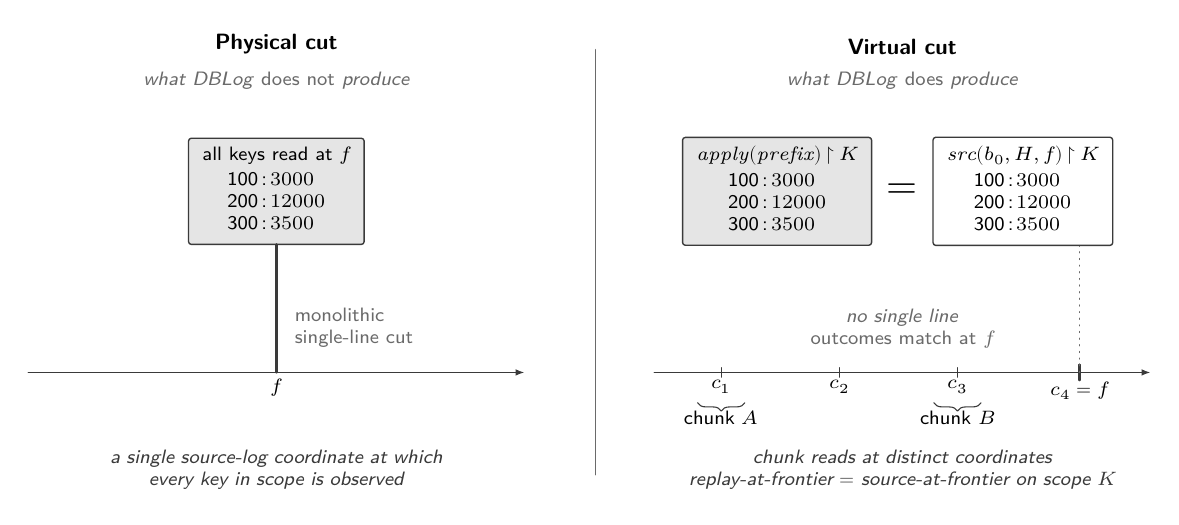
\begin{tikzpicture}[setA, x=1cm, y=1cm]

% ============================================================
% LEFT PANEL: Physical cut.
% Panel anchored at xshift=0.  Local x from 0..6.5.
% ============================================================
\begin{scope}[xshift=0cm]

% Panel title
\node[font=\sffamily\footnotesize\bfseries, anchor=south]
  at (3.25, 3.95) {Physical cut};
\node[font=\sffamily\scriptsize\itshape, text=gMid, anchor=south]
  at (3.25, 3.50) {what DBLog \emph{does not} produce};

% Source-log axis
\draw[axisLine] (0.10, 0) -- (6.40, 0);

\def\xF{3.25}

% State block above the cut.  Counterfactual: if DBLog produced a single
% physical cut, this is what it would deliver -- same target state as
% the right panel.  Concrete values reinforce "same outcome, different
% mechanism".  Centered at y=2.30 so the block aligns with the right
% panel's equality unit.
\node[blockFill, anchor=center, align=center,
      font=\sffamily\scriptsize, inner xsep=5pt, inner ysep=3pt]
  (lstate) at (\xF, 2.30) {%
  all keys read at $f$\\[1pt]
  \begin{tabular}{@{\ }r@{\,:\,}l@{\ }}
    100 & $3000$  \\
    200 & $12000$ \\
    300 & $3500$  \\
  \end{tabular}};

% Single thick cut line at f -- rises from the axis up to the
% state block's south edge.  Weight 0.9pt for cross-figure consistency.
\draw[gDark, line width=0.9pt] (\xF, 0) -- (lstate.south);
\node[font=\sffamily\scriptsize\bfseries, anchor=north, inner sep=1pt]
  at (\xF, -0.05) {$f$};

% Subtitle below the axis -- y=-0.70 so it aligns with the right panel.
\node[font=\sffamily\scriptsize\itshape, text=gDark, anchor=north,
      align=center, text width=58mm]
  at (\xF, -0.90)
  {a single source-log coordinate at which\\
   every key in scope is observed};

% Visual annotation: the cut LINE is what makes this "physical"
\node[font=\sffamily\scriptsize, anchor=west, text=gMid,
      align=left, inner sep=1pt]
  at (\xF+0.20, 0.55)
  {monolithic\\\strut single-line cut};

\end{scope}

% ============================================================
% VERTICAL DIVIDER between panels (stronger than gLight to read clearly)
% ============================================================
\draw[gMid, line width=0.5pt] (7.30, -1.30) -- (7.30, 4.10);

% ============================================================
% RIGHT PANEL: Virtual cut.
% Panel anchored at xshift=7.95cm.  Local x from 0..6.5.
% ============================================================
\begin{scope}[xshift=7.95cm]

% Panel title
\node[font=\sffamily\footnotesize\bfseries, anchor=south]
  at (3.25, 3.95) {Virtual cut};
\node[font=\sffamily\scriptsize\itshape, text=gMid, anchor=south]
  at (3.25, 3.50) {what DBLog \emph{does} produce};

% Source-log axis with c1..c4
\draw[axisLine] (0.10, 0) -- (6.40, 0);
\def\xCa{0.95}
\def\xCb{2.45}
\def\xCc{3.95}
\def\xCd{5.50}
\foreach \x/\lab in {\xCa/c_1, \xCb/c_2, \xCc/c_3} {
  \draw[axisTick] (\x, 0.06) -- (\x, -0.06);
  \node[font=\sffamily\scriptsize, anchor=north, inner sep=1pt]
    at (\x, -0.06) {$\lab$};
}
% Frontier tick c_4 = f, emphasized
\draw[axisTick, line width=0.8pt] (\xCd, 0.10) -- (\xCd, -0.10);
\node[font=\sffamily\scriptsize\bfseries, anchor=north, inner sep=1pt]
  at (\xCd, -0.08) {$c_4 = f$};

% Chunk-read brackets below axis
\draw[braceMirror] (\xCa-0.30, -0.35) -- (\xCa+0.30, -0.35);
\node[font=\sffamily\scriptsize, anchor=north, inner sep=1pt]
  at (\xCa, -0.45) {chunk $A$};
\draw[braceMirror] (\xCc-0.30, -0.35) -- (\xCc+0.30, -0.35);
\node[font=\sffamily\scriptsize, anchor=north, inner sep=1pt]
  at (\xCc, -0.45) {chunk $B$};

% Frontier guide -- dotted, rises from c_4 to the equality unit's bottom
\draw[guide] (\xCd, 0) -- (\xCd, 1.95);

% State boxes -- Apply == Src on K, anchored above the frontier
\def\eqY{2.30}
\node[font=\sffamily\Large, anchor=center] (eq) at (3.25, \eqY) {$=$};
\node[blockFill, anchor=east, align=center,
      font=\sffamily\scriptsize, left=3pt of eq.west,
      inner xsep=5pt, inner ysep=3pt]
  (lbox) {%
  \textbf{$\Apply(\CleanPrefix) \restrict K$}\\[1pt]
  \begin{tabular}{@{\ }r@{\,:\,}l@{\ }}
    100 & $3000$  \\
    200 & $12000$ \\
    300 & $3500$  \\
  \end{tabular}};
\node[block, anchor=west, align=center,
      font=\sffamily\scriptsize, right=3pt of eq.east,
      inner xsep=5pt, inner ysep=3pt]
  (rbox) {%
  \textbf{$\Src(b_0, H, f) \restrict K$}\\[1pt]
  \begin{tabular}{@{\ }r@{\,:\,}l@{\ }}
    100 & $3000$  \\
    200 & $12000$ \\
    300 & $3500$  \\
  \end{tabular}};

% Visual annotation: no single line gathers the keys
\node[font=\sffamily\scriptsize, anchor=center, text=gMid,
      align=center, inner sep=1pt]
  at (3.25, 0.55)
  {\emph{no single line}\\ outcomes match at $f$};

% Subtitle below the axis
\node[font=\sffamily\scriptsize\itshape, text=gDark, anchor=north,
      align=center, text width=58mm]
  at (3.25, -0.90)
  {chunk reads at distinct coordinates\\
   replay-at-frontier $=$ source-at-frontier on scope $K$};

\end{scope}

\end{tikzpicture}

\caption{Physical cut vs.\ virtual cut. \emph{Left:} a physical cut
requires a single source-log coordinate at which every key in scope is
observed, shown as a single vertical line. DBLog does \emph{not} produce
one. The values shown are the counterfactual outcome on $K$. \emph{Right:}
a virtual cut requires replay at the frontier to equal the source at
the frontier on the chosen scope. The chunk reads (as in
Figure~\ref{fig:running-example-timeline}) sit at distinct earlier
coordinates, no single line gathers them, and the equality lives in
outcome space rather than time space.}
\label{fig:virtual-vs-physical-cut}

\end{figure*}

This is the exact shape illustrated by the running example. There, the
replay sequence has seven items, the scope is
$\{100,200,300\}$, the frontier is $c_4$, and
$\Apply$ produces the same balances as $\Src$ at $c_4$
on those three keys. Chunk A and chunk B were read at different
coordinates; the virtual cut does not hide that fact. It says the replay
outcome is snapshot-equivalent on the claimed keys.

The state-level form is useful because Layer 2 proves the equality for
run accessors:

\[
  \VCS\bigl(\CleanPrefix(R),\Scope(R),\Frontier(R),H\bigr).
\]

Layer 3 then proves that an accepted certificate, under faithful source
observation, witnesses a run whose accessors agree with the certificate.
That is how the run-side theorem becomes the certificate-side theorem.

\section{Source-Side Virtual-Cut Soundness \mbox{(Layer 2)}}\label{source-side-virtual-cut-soundness-layer-2}

Layer 2 proves the source-side theorem:

\[
\begin{aligned}
  \WF(b_0,R,H) \,\Longrightarrow{}&
    \Apply(\CleanPrefix(R)) \restrict \Scope(R)\\
  &{}= \Src(b_0,H,\Frontier(R)) \restrict \Scope(R).
\end{aligned}
\]

Reader-facing theorem summary:

\begin{itemize}
\tightlist
\item
  \textbf{Status:} Conditional --- machine-checked under the displayed
  premises.
\item
  \textbf{Claim:} the clean prefix of a wellformed DBLog run reaches the
  source state at the run frontier on the run scope.
\item
  \textbf{Premises:} the wellformed-run obligations in
  Section~\ref{wellformed-runs},
  including chunk partition, CDC coverage and faithfulness, chunk-read
  honesty, and read-before-frontier discipline.
\item
  \textbf{Boundary:} this is a source-side run theorem, not yet a
  certificate, whole-table, or sink-state theorem.
\end{itemize}

Here, \textbf{Conditional} means machine-checked under the displayed
premises, not unproved or merely plausible.

Equivalently, every wellformed DBLog run satisfies the virtual-cut-state
equality at the run's frontier on the run's scope. The theorem is stated
about the run's raw clean prefix; by the window-suppression equivalence
of \S\ref{raw-replay-and-normalized-clean-prefix}, the normalized clean
prefix yields the same $\Apply$ state and therefore the same equality.

The theorem is \textbf{Conditional} on the wellformed-run model. That
does not mean the proof is informal. It means the proof assumes exactly
the wellformed-run predicate of
Section~\ref{wellformed-runs}: chunk partition, frontier
discipline, CDC coverage and faithfulness, and chunk-read honesty. Each
of these is visible because omitting it permits a real counterexample
(Table~\ref{tab:load-bearing-obligations}). The predicate's remaining
conjunct, clean-prefix closure, is instead definition-derived: it holds
for every run by the clean-prefix construction, so the proof may use it
but no deployment need establish it separately.

\subsection{Proof Idea}\label{proof-idea}

The proof is a per-key latest-event argument.

First, restricted-state equality reduces the theorem to pointwise
equality. It is enough to show that for every key $k$ in
$\Scope(R)$:

\[
  \Apply(\CleanPrefix(R))(k) = \Src(b_0,H,\Frontier(R))(k).
\]

Fix such a key $k$. Since the run is wellformed, $k$ has a
unique responsible chunk, and the chunk-read evidence produces a
value-or-absence refresh for $k$ that belongs to $\CleanPrefix(R)$,
including $\mathsf{Refresh}\,k\,\None\,c$ when the row is absent at the
chunk-read coordinate. Therefore the ``no replay event for $k$'' case
cannot occur for an in-scope key, and the clean-prefix-of-latest
correspondence --- the per-key step that says every in-scope $k$ has a
latest event in $\CleanPrefix(R)$, and that event is either a CDC event
or the responsible chunk's refresh --- collapses to the two cases below.

There are two real cases.

\subsection{Case 1: The Latest Replay Event Is
CDC}\label{case-1-the-latest-replay-event-is-cdc}

Suppose the latest replay event for $k$ in
$\CleanPrefix(R)$ is a CDC event $\mathsf{Cdc}\,c\,e$. The
clean-prefix coherence obligations say this replay event comes from an
observed CDC pair. CDC faithfulness says that observed pair is a real
source event in $H$; because the event lies in the clean prefix, its
source coordinate $c$ is within the run's frontier, i.e.\ $c \le
\Frontier(R)$. Order preservation and same-coordinate
multiplicity say the replay did not silently reverse or drop competing
source events for the same key and coordinate.

Now assume, for contradiction, that the source history has a later event
for $k$ at or before the frontier. CDC coverage would put that
later event into the observed CDC list. Clean-prefix closure would put
it into the replay. The clean-prefix ordering would place it after
$\mathsf{Cdc}\,c\,e$, contradicting the choice of $\mathsf{Cdc}\,c\,e$ as
the latest replay event for $k$.

So the latest replay CDC event corresponds to the latest source event
for $k$ through the frontier. $\Apply$ and $\Src$
therefore make the same update at $k$.

\subsection{Case 2: The Latest Replay Event Is a
Refresh}\label{case-2-the-latest-replay-event-is-a-refresh}

Suppose the latest replay event for $k$ is
$\mathsf{Refresh}\,k\,m\,c_{\mathit{read}}$. The responsible-chunk obligations
identify the chunk that produced it, and refresh honesty says:

\[
m = \Src(b_0,H,c_{\mathit{read}})(k).
\]

If there were a later source event for $k$ in
$(c_{\mathit{read}}, \Frontier(R)]$, CDC coverage and clean-prefix
closure would place a corresponding $\mathsf{Cdc}$ event after the refresh
in the clean prefix. The interval is open at $c_{\mathit{read}}$ because a
read at $c_{\mathit{read}}$ already observes source events at
$c_{\mathit{read}}$; the post-read repair obligation starts after the read
coordinate and runs through the frontier. A later source event would
contradict the refresh being latest for $k$.

Therefore the source state for $k$ at the read coordinate is
still the source state for $k$ at the frontier. The refresh
writes exactly that value or absence, so
$\Apply(\CleanPrefix(R))(k)$ equals
$\Src(b_0,H,\Frontier(R))(k)$. The value case and the
row-absence case use the same equation; absence is just $\None$ in
the per-key state.

\subsection{Why the Assumptions Are
Load-Bearing}\label{why-the-assumptions-are-load-bearing}

The proof fails if the obligations are weakened.

\begin{table*}[t]
\caption{Why selected obligations in $\WF$ are load-bearing:
counterexample shapes when the obligation is dropped, and the boundary
each clause protects.}
\label{tab:load-bearing-obligations}
\centering\small
\begin{tabularx}{\textwidth}{@{}p{1.4in}YY@{}}
\toprule
\textbf{Missing obligation} & \textbf{Counterexample shape} &
\textbf{Boundary protected}\\
\midrule
CDC coverage &
  A source update after a chunk read is missing from replay, so an old
  refresh wins. &
  DBLog needs retained source-log evidence.\\
Strict chunk ownership &
  Two chunks both claim a key, or no chunk owns it, so the refresh
  source is ambiguous or absent. &
  The theorem is scoped through a canonical chunk plan.\\
Read-before-frontier &
  A chunk read after the frontier injects a future value into the
  replay. &
  The replay is frontier-bound.\\
Same-coordinate order and multiplicity &
  Duplicate or same-coordinate source events are observed in a
  different order or with an occurrence missing. &
  Latest-event reasoning must match source order.\\
Refresh honesty &
  A chunk refresh records a value or absence that was not the source
  state at the read coordinate. &
  Chunk reads remain an External observation assumption.\\
Clean-prefix order &
  A clean-prefix event for some key sits before an earlier-coordinate
  same-key event, so the prefix's latest event for that key differs
  from the source's. &
  Per-key latest-event reasoning carries from the prefix to the
  source.\\
\bottomrule
\end{tabularx}
\end{table*}

These negative cases are not side decoration. They are why the theorem's
premise is the full wellformed-run predicate rather than a vague
statement that DBLog ``collected some chunks and some CDC.''

\smallskip
\noindent\textbf{Practitioner takeaway.} \emph{This is the paper's core
guarantee: a backfill that meets the wellformed-run obligations emits
chunk reads and CDC events that replay to exactly the source state at the
chosen frontier, on the chosen key scope --- with no table lock, no paused
writes, and no global read transaction. The result is scoped to that run;
the sections that follow add a checkable certificate and the side
conditions under which it lifts to the whole table.}

\section{Certificates, Evidence, and
Verifiers}\label{certificates-evidence-and-verifiers}

Layer 2 proves a theorem about an abstract DBLog run: if the run is
wellformed, its clean replay prefix reaches the source state at its
frontier on its scope. A deployment, however, does not hand a reader an
abstract run. It hands over a certificate and evidence. This section
explains the certificate-side vocabulary informally; Section~9 gives
the theorem and proof story.

\subsection{Certificate}\label{certificate}

A \textbf{certificate} is the claim object. It names:
\[
  \begin{aligned}
    \Scope(C)\quad        &\text{the keys being claimed},\\
    \Frontier(C)\quad      &\text{the source-log coordinate of the claim},\\
    \CleanPrefix(C)\quad   &\text{the certified replay prefix.}
  \end{aligned}
\]
The clean-prefix accessor is semantic. It is not a permission for a
serialized certificate to authenticate any arbitrary list of replay
events by storing it. The prefix becomes safe only when accepted
evidence materializes a wellformed run and ties the certificate
accessors to the run accessors. Before acceptance, $\CleanPrefix(C)$ is
only the \emph{claimed} prefix; the certificate theorem uses it only
after accepted evidence materializes a coherent wellformed run that
agrees with that accessor.

\subsection{Evidence}\label{evidence}

An \textbf{evidence bundle} contains the source-side material the
checker inspects: certificate binding evidence, the chunk plan,
chunk-read coordinates, chunk domains, observed row values or absences,
ordinary CDC observations, and the construction evidence for the raw or
normalized clean prefix.

The evidence bundle does not contain a destination-state proof. It does
not contain sink ACK semantics. It does not contain whole-table
claim-scope side conditions except where those are added later for the
whole-table specialization. The certificate layer is source-side.

\subsection{Materialized Run}\label{materialized-run}

The certificate theorem needs a bridge from artifact to model. That
bridge is the materialization relation $\Mat(C,E,R)$: certificate $C$
and evidence $E$ together describe the abstract DBLog run $R$ consumed
by the Layer~2 theorem. Materialization is structural --- it connects
the evidence to a run carrier with a scope, frontier, clean prefix,
chunk plan, chunk-read observations, and CDC observations --- but does
not by itself say that the run is wellformed against the source
history.

Concretely, $\Mat$ relates the pair to the evidence-determined run:
the materialized run's scope, frontier, clean prefix, chunk plan,
chunk-read observations, and CDC observations are fixed by what $E$
serializes, not chosen freely by the checker. Evidence that does not
describe a run shape the checker supports is reported $\Unsupported$
rather than carried into an accepted claim; the certificate's own
fields are tied to the materialized run by the coherence predicate
below.
Materialization adds no wellformedness and no faithfulness of its own;
that work is done by the coherence predicate and the checker-substrate
obligations, not hidden inside the bridge.

Rejected and unsupported evidence need not materialize any run. Accepted
evidence must not leave the checker free to choose an arbitrary
convenient run; that is exactly what the coherence predicate below
prevents.

\subsection{Certificate / Run
Coherence}\label{certificate-run-coherence}

We write $\Coh(C,E,R)$ for the certificate / run coherence predicate.
It packages materialization with accessor agreement between $C$ and
$R$:

\[
\begin{aligned}
\Coh(C,E,R) \,\Longleftrightarrow\,&
  \Mat(C,E,R)\\
  \land\,& \Scope(C)=\Scope(R)\\
  \land\,& \Frontier(C)=\Frontier(R)\\
  \land\,& \CleanPrefix(C)=\CleanPrefix(R).
\end{aligned}
\]

The evidence parameter is load-bearing. Coherence is not ``there exists
some run with matching accessors.'' It is about the run materialized by
this certificate/evidence pair.

\subsection{Verifier Result}\label{verifier-result}

The verifier result has three cases
(Table~\ref{tab:verifier-results}):

\begin{table}[t]
\caption{Verifier result cases.}
\label{tab:verifier-results}
\centering\small
\begin{tabularx}{\columnwidth}{@{}lY@{}}
\toprule
\textbf{Result} & \textbf{Meaning}\\
\midrule
$\Accept$ &
  The certificate/evidence pair is internally coherent for the
  source-side checker fragment.\\
$\Reject$ &
  The evidence contradicts the certificate or fails a required check.\\
$\Unsupported$ &
  The evidence uses source-side vocabulary outside the checker fragment
  modeled here.\\
\bottomrule
\end{tabularx}
\end{table}

$\Unsupported$ matters because silently ignoring unknown evidence
would be a soundness bug. If the checker cannot interpret an optional
source-side feature, the certificate is not accepted as if that feature
had been checked.

$\Accept$, $\Reject$, and $\Unsupported$ are verifier
results, not theorem-status labels. The verifier result here is an
abstract source-side checker result, not a claim that a serialized
certificate format, parser, or production verifier implementation has
been proved correct.

\subsection{What Accept Means, and What It Does Not
Mean}\label{what-accept-means-and-what-it-does-not-mean}

$\Accept$ means that, under faithful source observation, the
evidence materializes a wellformed DBLog run whose scope, frontier, and
clean prefix agree with the certificate. That is the bridge back to
Layer 2.

$\Accept$ does not mean that the database, connector, log,
primary-key interpretation, source-coordinate semantics, concrete
parser, wire format, or named product has been proved faithful by the
certificate itself. It does not mean a sink applied the prefix. It does
not mean the claim is whole-table. It does not remove the
faithful-source-observation premise.

\subsection{Faithful Source
Observation}\label{faithful-source-observation}

We write $\FSO(E,b_0,H,\RawObs)$ for the faithful-source-observation
assumption --- the External observation assumption of the certificate
layer. It ties the finite evidence bundle $E$ to the mathematical
source history $H$ and base state $b_0$, against a raw source-
observation carrier $\RawObs$. In practical terms it covers:

\begin{itemize}\tightlist
\item the source history and base state the certificate is about;
\item the meaning and ordering of source-log coordinates;
\item CDC retention and completeness over the certified interval;
\item preservation of same-coordinate order and multiplicity where
  relevant;
\item honesty of chunk-read values and absences at their recorded
  coordinates;
\item the primary-key interpretation and the assumption that chunk
  reads observe committed source state.
\end{itemize}

The theorem statements write the raw source-observation carrier as
$\RawObs$. $\RawObs$ is left abstract: it stands for whatever concrete
record a deployment has of what the source emitted, interpreted by the
faithful-source-observation assumption. It is not a destination log,
not a sink-state proof, and not a claim that a named connector has been
verified.

The certificate checker can compare evidence fields to one another. It
cannot prove, from the certificate alone, that the outside world
produced faithful observations. This is why the accepted-certificate
theorem is Conditional and why faithful source observation is labeled
as an External observation assumption.

\subsection{Why This Layer Exists}\label{why-this-layer-exists}

The certificate layer is the bridge from operational artifacts to the
theorem about replay equality. A wellformed run is the mathematical
object Layer 2 needs. A certificate is the artifact DBLog can expose.
The Layer 3 theorem says that accepted evidence gives enough of a bridge
from the artifact to the mathematical run, under the visible trust
boundary, for the source-side virtual-cut equality to follow.

\smallskip
\noindent\textbf{Practitioner takeaway.} \emph{A DBLog certificate is a
finite, checkable claim object --- scope, frontier, clean prefix ---
paired with an evidence bundle the checker inspects. Acceptance is an
internal coherence verdict, not a proof that the connector, log, or
parser is faithful: faithful source observation is part of every
accepted-certificate claim, not a footnote to it. Evaluating a
deployment means asking what its checker actually inspects and what it
instead has to assume.}

\section{Accepted-Certificate Soundness \mbox{(Layer 3)}}\label{accepted-certificate-soundness-layer-3}

Layer 3 gives the certificate-side theorem. It has two statements: an
intermediate bridge theorem and the composed virtual-cut theorem.

\subsection{Intermediate Theorem}\label{intermediate-theorem}

The intermediate theorem is \textbf{Conditional} on the \emph{checker
substrate}: a small set of primitive obligations the abstract
certificate checker must meet for acceptance to carry meaning.
Table~\ref{tab:checker-substrate} lists them. They are stated as
explicit assumptions; the paper does not prove a concrete parser, wire
format, or production verifier discharges them.

\begin{table}[t]
\caption{Checker-substrate obligations S1--S4: the conditional
structure of the accepted-certificate intermediate theorem.}
\label{tab:checker-substrate}
\centering\small
\begin{tabularx}{\columnwidth}{@{}l@{\hskip 1em}Y@{}}
\toprule
\textbf{} & \textbf{Checker-substrate obligation}\\
\midrule
S1 & Accepted inputs are wellformed checker inputs: structurally valid
     and parseable.\\
S2 & Accepted checker inputs materialize an abstract DBLog run.\\
S3 & The materialized run's accessors --- scope, frontier, and clean
     prefix --- agree with the certificate.\\
S4 & A faithful accepted materialization is a wellformed run against
     the source history.\\
\bottomrule
\end{tabularx}
\end{table}

Obligations S1--S4 are the conditional structure of the intermediate
theorem: each is a property of the checker design from which an
$\Accept$ return licenses the theorem's source-side conclusion.
Table~\ref{tab:checker-substrate} carries no fifth row because
Unsupported-evidence reporting is not part of that conditional list ---
it is a separate checker-design commitment, stated once outside the
table.

\smallskip
\noindent\textbf{Unsupported reporting.} A checker meeting S1--S4 must
also not accept evidence it cannot interpret as if it had been checked;
uninterpretable evidence is reported $\Unsupported$ rather than
$\Accept$. \textbf{Status:} Deployment obligation on the concrete
checker, not a Layer~3 premise.

Under obligations S1--S4 the intermediate theorem is:

\[
\begin{aligned}
&\Verify(C,E)=\Accept \,\land\, \FSO(E,b_0,H,\RawObs)\\
&\quad\Longrightarrow\, \exists R.\;
   \WF(b_0,R,H) \,\land\, \Coh(C,E,R).
\end{aligned}
\]

In words: accepted evidence, when interpreted through faithful source
observation, witnesses a wellformed abstract DBLog run whose accessors
agree with the certificate. Obligations S1--S3 carry the materialization
and accessor agreement, and S4 carries wellformedness. The
Unsupported-reporting commitment stated after the table is what keeps
uninterpretable evidence from being accepted as if it had been checked;
it is operational, not part of the conditional list.

\subsection{Composed Theorem}\label{composed-theorem}

The headline certificate theorem is:

\[
\begin{aligned}
&\Verify(C,E)=\Accept \,\land\, \FSO(E,b_0,H,\RawObs)\\
&\quad\Longrightarrow\, \VC(C,H).
\end{aligned}
\]

Expanded:

\[
\begin{aligned}
&\Verify(C,E)=\Accept \,\land\, \FSO(E,b_0,H,\RawObs)\\
&\quad\Longrightarrow
  \Apply(\CleanPrefix(C)) \restrict \Scope(C)\\
&\qquad= \Src(b_0,H,\Frontier(C)) \restrict \Scope(C).
\end{aligned}
\]

Reader-facing theorem summary:

\begin{itemize}
\tightlist
\item
  \textbf{Status:} Conditional --- machine-checked under
  checker-substrate obligations S1--S4 (Table~\ref{tab:checker-substrate})
  and faithful source observation.
\item
  \textbf{Claim:} an accepted certificate is a virtual-cut certificate
  when its evidence is interpreted through faithful source observation.
\item
  \textbf{Premises:} checker-substrate obligations S1 (input
  wellformedness), S2 (materialization), S3 (accessor agreement),
  S4 (faithful materialization is wellformed); and faithful source
  observation of the evidence.
\item
  \textbf{Boundary:} acceptance does not prove a concrete parser, wire
  format, production verifier, named product, whole-table claim, or sink
  application. The Unsupported-reporting commitment is a separate
  checker-design obligation, not part of the conditional list.
\end{itemize}

Here, \textbf{Conditional} means machine-checked under obligations
S1--S4 and faithful source observation, not unproved or merely
plausible.

This is the formal meaning of ``an accepted DBLog certificate is a
virtual-cut certificate.'' The faithful-source-observation premise is
part of the sentence, not a footnote. Acceptance alone is not a proof
about the mathematical source history.

\subsection{Proof Explanation}\label{proof-explanation}

The proof composes the layers already introduced.

First, verifier acceptance and faithful source observation produce a
witnessed run $R$:

\[
\begin{aligned}
&\WF(b_0,R,H),\\
&\Coh(C,E,R).
\end{aligned}
\]

Second, Layer 2 applies to that wellformed run:

\[
\begin{aligned}
&\Apply(\CleanPrefix(R)) \restrict \Scope(R)\\
&\qquad= \Src(b_0,H,\Frontier(R)) \restrict \Scope(R).
\end{aligned}
\]

Third, coherence substitutes certificate accessors for run accessors:

\[
\begin{aligned}
\Scope(C)&=\Scope(R),\\
\Frontier(C)&=\Frontier(R),\\
\CleanPrefix(C)&=\CleanPrefix(R).
\end{aligned}
\]

After substitution, the Layer 2 equality becomes:

\[
\begin{aligned}
&\Apply(\CleanPrefix(C)) \restrict \Scope(C)\\
&\qquad= \Src(b_0,H,\Frontier(C)) \restrict \Scope(C).
\end{aligned}
\]

Fourth, Section~6's definition folds that equality into
$\VC(C,H)$.

No sink premise appears in this proof. No whole-table premise appears in
this proof. No named product premise appears in this proof. The proof is
scoped to $\Scope(C)$, source-side, and conditional on the checker
substrate and faithful source observation.

\subsection{Non-Vacuity and Boundary
Cases}\label{non-vacuity-and-boundary-cases}

The certificate layer is not only a theorem statement. The paper also
checks that the statement is meaningful:

\begin{itemize}\tightlist
\item there is a nonempty accepted-certificate witness with a
  non-base frontier, a chunk read, a value-changing replay event, and
  faithful $\RawObs$/$b_0$/$H$ evidence;
\item accepted-without-witness shapes are rejected by the
  checker-substrate obligations;
\item wrong certificate/evidence binding is rejected;
\item unknown source-side evidence is $\Unsupported$ rather than
  silently accepted;
\item mismatched certificate/run accessors fail coherence;
\item unfaithful $\RawObs$, wrong $b_0$, and wrong $H$ fail faithful
  source observation;
\item empty scope is a trivial boundary, not the positive witness.
\end{itemize}

These cases protect the main trust boundary. The theorem does not say
that the certificate eliminates trust. It says that, under faithful
source observation and explicit checker obligations, acceptance gives a
coherent wellformed run; the already-proved source-side theorem then
yields the certified virtual cut.

\smallskip
\noindent\textbf{Practitioner takeaway.} \emph{Rather than trusting a
backfill pipeline end to end, a consumer can check a finite certificate
against its evidence bundle. Acceptance is not self-authenticating: under
explicit checker obligations it yields the virtual cut only given
faithful source observation --- that the captured evidence honestly
reflects the real source --- which no verifier can settle from inside the
certificate.}

\section{Whole-Table Specialization \mbox{(Layer 4)}}\label{whole-table-specialization-layer-4}

Layers 2 and 3 prove a scoped result: the certified clean prefix reaches
the source state at the certified frontier on $\Scope(C)$. That is
the right headline for ordinary DBLog certificates, because a backfill
usually claims a finite key scope. That scope is in practice often the
whole table or a whole shard, so the whole-table side conditions below
are not an exotic case --- they are what a typical full backfill must
discharge. A whole-table statement needs more.
It needs evidence that the claimed scope really covers every table key
whose state could matter between a chosen anchor boundary and the
certified frontier, and it needs the replay prefix not to mutate keys
outside that claim.

The whole-table specialization is therefore a derived result, not a new
meaning of certificate acceptance. Acceptance gives the scoped virtual
cut. The additional side condition tells us when the restriction to
$\Scope(C)$ can be dropped.

\subsection{Anchor Boundary and Anchor
Domain}\label{anchor-boundary-and-anchor-domain}

An anchor boundary $b$ is a source coordinate used to name the
table population the whole-table claim intends to cover. It is not a
physical snapshot read. Chunks may be read after $b$; the
virtual-cut construction is precisely that stale chunk observations can
be repaired by source-log evidence and replayed to the frontier.

For a certificate $C$, the anchor must not be later than the
certified frontier:

\[
b \le \Frontier(C).
\]

The anchor domain is the set of keys present in the source at that
boundary:

\[
  \AnchorDomain(H,b)
    = \{\,k \mid \Src(b_0,H,b)(k) \text{ is present}\,\}.
\]

The anchor domain inherits its dependence on the base state $b_0$ from
$\Src$. As with $\Src$, $b_0$ is a single base state fixed throughout the
paper; we keep it implicit in $\AnchorDomain(H,b)$, and likewise in the
whole-table claim scope $\WTS(C,H,b)$ below, since it never varies. A
key present at the anchor that no source event at or before $b$ ever
writes owes its anchor-domain membership entirely to $b_0$ --- the one
place the base state does observable work in a whole-table claim.

Operationally, a whole-table deployment may use a maximum-primary-key
or equivalent end-of-table witness to help show that the claimed scope
covers this anchor domain. Such a witness does not replace $\WTS$: it
must be tied to the anchor boundary $b$, or otherwise justify
$\AnchorDomain(H,b) \subseteq \Scope(C)$. It also does not discharge the
post-anchor touch condition below, including for keys beyond an
anchor-time maximum.

Keys absent at $b$ can still become relevant later. If the source
inserts, updates, or deletes a key after $b$ and at or before the
certified frontier, the whole-table claim must account for that key too.

$\TouchedBetween(H,b,f)$ is the set of keys $k$ for which $H$
has an insert, update, or delete at some source coordinate $c$
with $b < c \le f$, and the conservative interval table scope is
\[
\begin{aligned}
&\TableScopeBetween(H,b,f)\\
&\quad= \AnchorDomain(H,b) \cup \TouchedBetween(H,b,f).
\end{aligned}
\]

This is a conservative event-touch scope. It is not a minimal
semantic-difference set: even a delete of an already absent key is still
a touch that the whole-table side condition can require the claim scope
to cover.

\subsection{A Small Anchor Example}\label{a-small-anchor-example}

Suppose the source contains keys $100$ and $200$ at anchor
boundary $b$. Between $b$ and frontier $f$, key
$300$ is inserted and key $200$ is deleted.

\[
\begin{aligned}
\AnchorDomain(H,b)&=\{100,200\},\\
\TouchedBetween(H,b,f)&=\{200,300\},\\
\TableScopeBetween(H,b,f)&=\{100,200,300\}.
\end{aligned}
\]

A whole-table claim for this interval must include all three keys in
$\Scope(C)$. Key $100$ is present at the anchor. Key
$200$ is present at the anchor and then deleted. Key $300$
is absent at the anchor but inserted before the frontier. Omitting any
of them would make the whole-table statement stronger than the evidence
supports.

There is also a replay-side condition. If the certified clean prefix
writes a bystander key $999$ outside $\Scope(C)$, then
scoped equality over $\{100,200,300\}$ may still be true, but
whole-table equality is not justified: the replay has changed something
outside the claimed table scope.

\subsection{Whole-Table Claim Scope}\label{whole-table-claim-scope}

We write $\WTS(C,H,b)$ for the whole-table claim-scope side condition.
It bundles four conjuncts:

\[
\begin{aligned}
&\WTS(C,H,b) \,\Longleftrightarrow\, b \le \Frontier(C)\\
&\,\land\, \AnchorDomain(H,b) \subseteq \Scope(C)\\
&\,\land\, \TouchedBetween(H,b,\Frontier(C)) \subseteq \Scope(C)\\
&\,\land\, \ReplayKeys(\CleanPrefix(C)) \subseteq \Scope(C).
\end{aligned}
\]

The first conjunct fixes the ordering of the anchor and frontier. The
next two say that $\Scope(C)$ covers every key present at the
anchor and every key touched after the anchor through the frontier. The
final conjunct says that the certified replay prefix does not write
unclaimed keys.
Figure~\ref{fig:whole-table-claim-scope} pictures the four conjuncts as
overlapping key regions (anchor-domain, touched-between, replay-keys)
over the source-coordinate axis.

\begin{figure*}[t]
  % fig05.tex -- Set A (Architectural) Figure 5: Anchor domain and
% whole-table claim scope.
%
% Cleaner integrated diagram: outer scope(C) rounded rectangle with
% generous interior; ellipse names placed ABOVE each ellipse (outside,
% inside the rectangle); concrete keys inside each ellipse; source-log
% axis below; four numbered conjuncts as circled numerals.

\centering
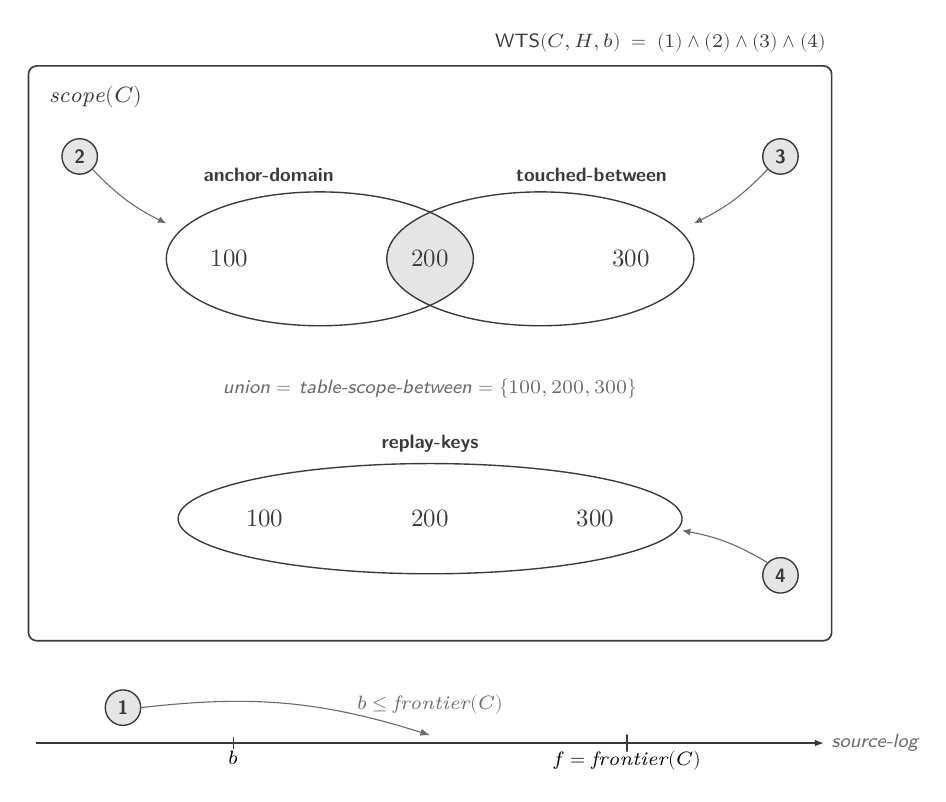
\begin{tikzpicture}[setA, x=1cm, y=1cm,
    conjNum/.style={
      draw=gDark, line width=0.5pt, circle, fill=gPale,
      minimum size=4.5mm, inner sep=0pt, font=\sffamily\bfseries\scriptsize,
      text=gDark,
    },
    keyDot/.style={
      font=\sffamily\small\bfseries, text=gDark, inner sep=1pt,
    },
    ellOutline/.style={gDark, line width=0.5pt},
    ellName/.style={font=\sffamily\scriptsize\bfseries, text=gDark, inner sep=1pt},
  ]

% ============================================================
% Outer scope(C) rectangle -- taller now, more breathing room.
% ============================================================
\def\rectXmin{0}
\def\rectXmax{10.20}
\def\rectYmin{0}
\def\rectYmax{7.3}
\def\axisY{-1.30}

\draw[gDark, line width=0.6pt, rounded corners=3pt]
  (\rectXmin, \rectYmin) rectangle (\rectXmax, \rectYmax);

% scope(C) header label, inset inside the top-left corner so the
% rounded rectangle border draws intact behind it.
\node[font=\sffamily\bfseries\footnotesize, anchor=north west, inner sep=4pt,
      text=gDark]
  at (\rectXmin+0.12, \rectYmax-0.12) {$\Scope(C)$};

% ============================================================
% Upper region: anchor-domain and touched-between ellipses.
% Labels sit ABOVE each ellipse (still inside the rectangle).
% ============================================================
\def\anchorCx{3.7}
\def\anchorCy{4.85}
\def\touchedCx{6.5}
\def\touchedCy{4.85}
\def\ellRx{1.95}
\def\ellRy{0.85}

\node[ellName, anchor=south]
  at (\anchorCx-0.65, \anchorCy+\ellRy+0.10) {anchor-domain};
\node[ellName, anchor=south]
  at (\touchedCx+0.65, \touchedCy+\ellRy+0.10) {touched-between};

% Intersection of the two ellipses, filled with gPale to make the
% Venn overlap visually obvious (200 sits in this lens region).
\begin{scope}
  \clip (\anchorCx, \anchorCy) ellipse [x radius=\ellRx, y radius=\ellRy];
  \fill[gPale] (\touchedCx, \touchedCy) ellipse [x radius=\ellRx, y radius=\ellRy];
\end{scope}

\draw[ellOutline]
  (\anchorCx, \anchorCy) ellipse [x radius=\ellRx, y radius=\ellRy];
\draw[ellOutline]
  (\touchedCx, \touchedCy) ellipse [x radius=\ellRx, y radius=\ellRy];

% Keys inside the ellipses
\node[keyDot] at (\anchorCx-1.15, \anchorCy)   {$100$};
\node[keyDot] at ($(\anchorCx, \anchorCy)!0.5!(\touchedCx, \touchedCy)$) {$200$};
\node[keyDot] at (\touchedCx+1.15, \touchedCy) {$300$};

% Union annotation between upper and lower ellipses
\node[font=\sffamily\scriptsize\itshape, text=gMid, anchor=center,
      align=center, inner sep=2pt]
  at (5.10, 3.20)
  {union $=$ table-scope-between $= \{100, 200, 300\}$};

% ============================================================
% Lower region: replay-keys ellipse.
% Label sits ABOVE it (inside the rectangle).
% ============================================================
\def\replayCx{5.10}
\def\replayCy{1.55}
\def\replayRx{3.2}
\def\replayRy{0.70}

\node[ellName, anchor=south]
  at (\replayCx, \replayCy+\replayRy+0.10) {replay-keys};

\draw[ellOutline]
  (\replayCx, \replayCy) ellipse [x radius=\replayRx, y radius=\replayRy];

\node[keyDot] at (\replayCx-2.10, \replayCy) {$100$};
\node[keyDot] at (\replayCx,      \replayCy) {$200$};
\node[keyDot] at (\replayCx+2.10, \replayCy) {$300$};

% ============================================================
% Source-log axis BELOW the rectangle.
% ============================================================
\draw[axisLine] (0.10, \axisY) -- (10.10, \axisY);
\node[sublabelDim, anchor=west, inner sep=0pt]
  at (10.20, \axisY) {source-log};

\def\bX{2.60}
\def\fX{7.60}
\draw[axisTick] (\bX, \axisY+0.07) -- (\bX, \axisY-0.07);
\node[font=\sffamily\scriptsize, anchor=north, inner sep=1pt]
  at (\bX, \axisY-0.07) {$b$};
\draw[axisTick, line width=0.8pt] (\fX, \axisY+0.10) -- (\fX, \axisY-0.10);
\node[font=\sffamily\scriptsize\bfseries, anchor=north, inner sep=1pt]
  at (\fX, \axisY-0.07) {$f = \Frontier(C)$};

% Relation b <= f.  Lifted to y+0.30 so the conjunct-(1) leader (which
% lands at y+0.10) clears it.
\node[font=\sffamily\scriptsize\itshape, text=gMid, anchor=south, inner sep=2pt]
  at ($(\bX, \axisY)!0.5!(\fX, \axisY) + (0, 0.30)$) {$b \le \Frontier(C)$};

% ============================================================
% Conjunct circled numerals.
% ============================================================
% (1) lifted slightly above the axis, with a leader pointing to the
% interval between b and f (the relation, not the point b alone).
\node[conjNum] (c1n) at (\bX-1.40, \axisY+0.45) {1};
\draw[depFlow, line width=0.4pt]
  (c1n.east) to[bend left=12]
  ($(\bX, \axisY)!0.5!(\fX, \axisY) + (0, 0.10)$);

% (2) upper-left, leader into anchor-domain ellipse.
% Pinned at absolute Y=6.15 so the rectYmax bump doesn't push it
% closer to the scope(C) header above.
\node[conjNum] (c2n) at (\rectXmin+0.65, \rectYmax-1.15) {2};
\draw[-{Latex[length=3pt, width=2.5pt]}, gMid, line width=0.4pt]
  (c2n.south east) to[bend right=10] ($(\anchorCx-\ellRx, \anchorCy+0.45)$);

% (3) upper-right, leader into touched-between.  Same pinning as (2).
\node[conjNum] (c3n) at (\rectXmax-0.65, \rectYmax-1.15) {3};
\draw[-{Latex[length=3pt, width=2.5pt]}, gMid, line width=0.4pt]
  (c3n.south west) to[bend left=10] ($(\touchedCx+\ellRx, \touchedCy+0.45)$);

% (4) lower-right, leader into replay-keys
\node[conjNum] (c4n) at (\rectXmax-0.65, \rectYmin+0.83) {4};
\draw[-{Latex[length=3pt, width=2.5pt]}, gMid, line width=0.4pt]
  (c4n.north west) to[bend right=10] ($(\replayCx+\replayRx, \replayCy-0.15)$);

% ============================================================
% Header summarizing the predicate as a 4-conjunct AND.
% Sits ABOVE the rectangle, right-aligned.
% ============================================================
\node[font=\sffamily\scriptsize, text=gDark, anchor=south east, align=right,
      inner sep=2pt]
  at (\rectXmax, \rectYmax+0.10) {%
  \textbf{$\WholeTableClaimScope(C, H, b) \;=\;
          (1) \land (2) \land (3) \land (4)$}};

\end{tikzpicture}

\caption{Anchor domain and whole-table claim scope. The four numbered
conjuncts of $\WholeTableClaimScope(C, H, b)$ are annotated on the
diagram. The base state $b_0$, fixed by context, is implicit in
$\WholeTableClaimScope$ and $\AnchorDomain$. \textbf{(1)} The anchor $b$ precedes the frontier on the
source-log axis: $b \le \Frontier(C)$.
\textbf{(2)} $\AnchorDomain(H, b) \subseteq \Scope(C)$.
\textbf{(3)} $\TouchedBetween(H, b, \Frontier(C)) \subseteq \Scope(C)$.
\textbf{(4)} $\ReplayKeys(\CleanPrefix(C)) \subseteq \Scope(C)$.
Concrete keys follow the worked example of Section~\ref{a-small-anchor-example}: $100$ sits in
anchor-domain only, $200$ in the overlap, $300$ in touched-between
only. Replay-keys are $\{100, 200, 300\}$.}
\label{fig:whole-table-claim-scope}

\end{figure*}

This predicate is explicit because whole-table correctness is not
automatic. Certificate acceptance alone gives a scoped statement. The
whole-table side condition is the extra bridge from ``correct on the
certified claim scope'' to ``correct on every table key''.

\subsection{Whole-Table Theorem}\label{whole-table-theorem}

Under certificate acceptance, faithful source observation, and the
whole-table claim-scope side condition, the certified clean prefix
reaches the source state at the certified frontier on the whole table:

\[
\begin{aligned}
&\Verify(C,E)=\Accept \,\land\, \FSO(E,b_0,H,\RawObs)\\
&\,\land\, \WTS(C,H,b)\\
&\,\Longrightarrow\, \Apply(\CleanPrefix(C))=\Src(b_0,H,\Frontier(C)).
\end{aligned}
\]

Reader-facing theorem summary:

\begin{itemize}
\tightlist
\item
  \textbf{Status:} Conditional --- machine-checked under
  checker-substrate obligations S1--S4
  (Table~\ref{tab:checker-substrate}), faithful source observation,
  and $\WTS(C,H,b)$.
\item
  \textbf{Claim:} the scoped certificate theorem lifts to whole-table
  source-state equality when the whole-table claim-scope side conditions
  cover boundary order, anchor-domain keys, post-anchor touches, and
  replay keys.
\item
  \textbf{Premises:} certificate acceptance, faithful source
  observation, $\WTS(C,H,b)$, and checker-substrate obligations
  S1--S4 (Table~\ref{tab:checker-substrate}).
\item
  \textbf{Boundary:} this remains source-side. It does not prove sink
  convergence, exactly-once delivery, or arbitrary destination
  correctness.
\end{itemize}

This is a \textbf{Conditional} source-side theorem. The certificate
checker and faithful-source-observation assumption supply the certified
scoped virtual cut; the whole-table side condition supplies the coverage
needed to remove the scope restriction.

\subsection{Proof Roadmap}\label{proof-roadmap}

Layer 3 gives the scoped equality:

\[
\begin{aligned}
&\Apply(\CleanPrefix(C)) \restrict \Scope(C)\\
&\,= \Src(b_0,H,\Frontier(C)) \restrict \Scope(C).
\end{aligned}
\]

For keys inside $\Scope(C)$, that is already the desired equality.
For keys outside $\Scope(C)$, the whole-table side condition does
two jobs. The $\WTS(C,H,b)$ inclusions
\[
  \begin{aligned}
    \AnchorDomain(H,b)                &\subseteq \Scope(C), \\
    \TouchedBetween(H,b,\Frontier(C)) &\subseteq \Scope(C), \\
    \ReplayKeys(\CleanPrefix(C))      &\subseteq \Scope(C)
  \end{aligned}
\]
contrapose to
$k \notin \Scope(C) \Rightarrow k \notin \AnchorDomain(H,b)$,
$k \notin \Scope(C) \Rightarrow
  k \notin \TouchedBetween(H,b,\Frontier(C))$, and
$k \notin \Scope(C) \Rightarrow k \notin \ReplayKeys(\CleanPrefix(C))$,
which power the two cases. First, the $b_0$-aware anchor-domain
definition makes absence outside the anchor domain mean absence at the
anchor boundary, including keys from the base state. Together with
$b \le \Frontier(C)$ and no post-anchor touch through the frontier,
this implies the key is absent from the source at the frontier.
Second, because the key is outside $\ReplayKeys(\CleanPrefix(C))$, the
clean prefix does not write it. Replay and source are therefore both
absent outside $\Scope(C)$. Combining the inside-scope and
outside-scope cases gives unrestricted equality.

\subsection{Boundaries}\label{boundaries}

The specialization does not change the paper's trust boundaries. It
still depends on faithful observation of the source-side evidence. It
does not prove that a concrete parser or production verifier
implementation is correct. It does not prove sink-state convergence,
exactly-once delivery, or arbitrary destination correctness. It also
does not say that a virtual cut is a physical cut: the anchor is a
source-coordinate boundary used for reasoning about table scope, not a
single request-wide read timestamp.

\smallskip
\noindent\textbf{Practitioner takeaway.} \emph{A scoped certificate
becomes a whole-table guarantee only when the claimed key scope covers
every key present at the anchor boundary and every key touched between
the anchor and the frontier --- post-anchor inserts and deletes
included --- and the certified replay writes nothing outside that scope.
Whole-table correctness is earned by discharging those side conditions;
certificate acceptance alone does not grant it.}

\section{Source-Side Continuation and Restriction of Virtual
Cuts}\label{source-side-continuation-and-restriction}

The theorem ladder so far certifies a virtual cut at one frontier. A
certificate fixes a single frontier $\Frontier(C)$ and proves replay
equality there. But a DBLog deployment does not stop at that frontier.
The backfill chunk loop is finite, and once it closes DBLog keeps
running as ordinary change-data-capture, consuming source-log events as
the source commits them. The certified virtual cut is therefore one
observation of an ongoing process, not its end state.

This section proves two source-side algebra facts that connect
point-in-time cuts into that ongoing process. \emph{Continuation across
frontiers} shows that a virtual cut at frontier $f$ extends to a virtual
cut at any later frontier $f'$ by appending the faithful change-data
segment the source committed in between. \emph{Restriction to a
sub-scope} shows that a virtual cut on a key scope $K$ is also a virtual
cut on any smaller scope. Together they make the informal reading
precise: ongoing DBLog operation is a \emph{sequence} of virtual cuts,
each later cut obtained from an earlier one by appending a continuation
segment.

The Future Work section lists
continuation across frontiers and restriction to a sub-scope among the
goals of a wider certificate-algebra program
(Section~\ref{certificate-algebra-and-model-extensions}). This section discharges
those two as machine-checked results; the remaining program ---
disjoint composition, concrete extended-certificate verification, and
raw overlap/retry normalization --- stays Future work. Every result
here is source-side: each conclusion is again an
$\Apply$-against-$\Src$ equality on a scope, with no destination,
replica, or delivery term.

\smallskip
\noindent\emph{Proof roadmap.} Both theorems are proved pointwise per
key. Continuation across frontiers rests on one new Layer~0 fact --- the
source state at a later frontier is fixed by the source state at the
earlier frontier together with the events strictly between them
(\S\ref{layer-0-and-layer-1-lemmas}) --- while restriction to a
sub-scope is immediate from the per-key form of the virtual-cut
equality. The section defines the continuation segment first, then
proves the two theorems and a certificate-level corollary.

\subsection{Continuation Segments}\label{continuation-segments}

Continuation needs a precise object for ``the change data the source
committed between two frontiers.'' We call it the continuation segment.

For a source history $H$, a key scope $K$, and source frontiers
$f \le f'$, the continuation segment for the half-open interval
$(f,f']$ on $K$ is built directly from the source history: keep every
history event whose source coordinate $c$ satisfies $f < c \le f'$ and
whose key lies in $K$, in source order, and read each kept event as its
CDC replay event. We write $\ContSeg(H,K,f,f',\delta)$ for the
predicate ``$\delta$ is that continuation segment.'' By exact coverage,
$\delta$ contains \emph{exactly} the change-data readings of the source
events for keys in $K$ on $(f,f']$ --- no more, no less --- preserving
per-key order and multiplicity; this bidirectional equivalence between
$\delta$ and the source's own interval events is what the predicate
encodes by construction.

By construction, $\ContSeg(H,K,f,f',\delta)$ entails $f \le f'$: the
predicate is false whenever $f > f'$, independent of $\delta$. Theorems
whose premises include $\ContSeg(H,K,f,f',\delta)$ therefore implicitly
require $f \le f'$; the order is not restated in their displayed
formulas.

The interval is half-open because the coordinate convention is
inclusive (Section~\ref{source-histories-and-frontiers}):
$\Src(b_0,H,f)$ already reflects every event at coordinate $f$, so a
continuation starts strictly after $f$ and runs through $f'$ inclusive.

Defining the segment as \emph{the filtered source history, read as
change data} --- rather than as ``some list of CDC events between $f$
and $f'$'' --- is deliberate. It fixes source order, same-coordinate
source-position order, and event multiplicity by construction. A caller
cannot present a segment that quietly reorders, drops, or duplicates the
source's own events; any such list simply fails to be
$\ContSeg(H,K,f,f',\delta)$. That a real CDC feed delivers exactly this
segment is an \textbf{External observation assumption}, with a matching
\textbf{Deployment obligation} to retain the source-log interval
$(f,f']$ --- the same trust boundary the certificate layer already
names for chunk reads, now applied to the continuation.

The segment is filtered to the scope $K$: it is the change data for
the keys of $K$, not the source's entire change stream. A deployment
whose CDC feed carries all keys must project that stream onto $K$ to
obtain the continuation segment for a $K$-scoped cut; for a
whole-table continuation the scope is the universal key set, and the
whole-table continuation result below is the form to use. The
exactness cuts two ways. A segment that drops, reorders, or duplicates
an \emph{in-scope} event is not $\ContSeg(H,K,f,f',\delta)$ and the
continuation does not hold --- these are the proof-critical clauses. A
segment padded with an \emph{out-of-scope} event also fails
$\ContSeg$, but that rejection is evidence-shaping discipline rather
than soundness: the scoped equality constrains only the keys of $K$.

\subsection{Continuation Across
Frontiers}\label{continuation-across-frontiers}

The primary theorem of this section continues a virtual cut to a later
frontier. Let $H$ be a wellformed source history. If $\sigma$ is a
virtual cut at frontier $f$ on scope $K$, and $\delta$ is the
continuation segment for $(f,f']$ on $K$, then $\sigma$ followed by
$\delta$ --- sequence concatenation, written $\sigma \mathbin{@} \delta$
--- is a virtual cut at the later frontier $f'$ on the same scope:

\[
\begin{aligned}
&H \text{ wellformed} \,\land\, \VCS(\sigma,K,f,H)\\
&\,\land\, \ContSeg(H,K,f,f',\delta)\\
&\,\Longrightarrow\, \VCS(\sigma \mathbin{@} \delta, K, f', H).
\end{aligned}
\]

Reader-facing theorem summary:

\begin{itemize}
\tightlist
\item
  \textbf{Status:} Conditional --- machine-checked under the displayed
  premises.
\item
  \textbf{Claim:} appending the faithful continuation segment for
  $(f,f']$ carries a virtual cut at $f$ to a virtual cut at $f'$ on the
  same scope.
\item
  \textbf{Premises:} $H$ is a wellformed source history; $\sigma$ is a
  virtual cut at $f$ on $K$; and $\delta$ is exactly the continuation
  segment for $(f,f']$ on $K$.
\item
  \textbf{Boundary:} the conclusion is a replay-against-source equality
  on $K$. It is not a whole-table claim, not a statement that a verifier
  accepts an extended certificate, and not a destination-apply claim.
\end{itemize}

The wellformedness premise is not decorative. The proof needs the
source history's coordinate order to know that the events in $(f,f']$
are exactly the ones between the two frontiers; without it the interval
could interleave with events outside it.

\emph{Proof idea.} The argument is pointwise on a key $k \in K$. Replay
of a sequence at $k$ is fixed by the latest replay event for $k$. If the
continuation segment $\delta$ carries an event for $k$, then the latest
$k$-event of $\sigma \mathbin{@} \delta$ lies in $\delta$ and is the
change-data reading of the latest source event for $k$ in $(f,f']$; a
Layer~0 source-state interval lemma equates that event's effect with
$\Src(b_0,H,f')$ at $k$. If $\delta$ carries no event for $k$, replay of
$\sigma \mathbin{@} \delta$ at $k$ equals replay of $\sigma$ at $k$,
which the premise equates with $\Src(b_0,H,f)$ at $k$; the same interval
lemma equates that with $\Src(b_0,H,f')$ at $k$, because no event for
$k$ in the interval means the source state for $k$ does not change
across it. The interval lemma --- that $\Src$ at $f'$ is determined by
$\Src$ at $f$ together with the source events in $(f,f']$ --- is the one
new Layer~0 fact the continuation needs; it is proved from the
source-coordinate order.

\smallskip
\noindent\textbf{Whole-table continuation.} The whole-table
specialization (Section~\ref{whole-table-specialization-layer-4})
delivers, under its claim-scope side conditions, the \emph{unrestricted}
equality $\Apply(\sigma) = \Src(b_0,H,f)$. Continuation specializes to
that case: for a wellformed $H$, if $\Apply(\sigma) = \Src(b_0,H,f)$
holds on every key and $\delta$ is the continuation segment for
$(f,f']$ on every key, then
$\Apply(\sigma \mathbin{@} \delta) = \Src(b_0,H,f')$. This is the
all-keys instance of the theorem above, \textbf{Conditional} on the same
premises. It does not let a \emph{scoped} continuation become
whole-table for free: a key the source inserts outside $K$ within
$(f,f']$ changes the table while leaving the scoped equality on $K$
intact. Whole-table continuation requires the continuation segment for
every key, just as whole-table specialization requires its claim-scope
side condition.

\subsection{Restriction to a
Sub-Scope}\label{restriction-to-a-sub-scope}

A virtual cut also restricts downward along the scope. If $\sigma$ is a
virtual cut at frontier $f$ on scope $K$, then it is a virtual cut at
$f$ on every sub-scope $K' \subseteq K$:

\[
\VCS(\sigma,K,f,H) \,\land\, K' \subseteq K
  \,\Longrightarrow\, \VCS(\sigma,K',f,H).
\]

This is \textbf{Conditional} and premise-bearing: it holds for any
$K' \subseteq K$, and the $K' \subseteq K$ premise is exactly what it
needs. Restriction is one-directional. \emph{Widening} a scope is
unsound: for a key outside $K$ the cut certifies nothing about that
key's state at $f$, so there is no sound lemma carrying a cut from $K$
to a larger scope.

The same fact holds through a certificate's accessors. If $C$ is a
certificate with $\VC(C,H)$ and $K' \subseteq \Scope(C)$, then the
certified clean prefix is a virtual cut at $\Frontier(C)$ on the
narrowed scope $K'$:

\[
\begin{aligned}
&\VC(C,H) \,\land\, K' \subseteq \Scope(C)\\
&\quad\Longrightarrow\,
  \VCS\bigl(\CleanPrefix(C),K',\Frontier(C),H\bigr).
\end{aligned}
\]

This restricts the \emph{equality} a certificate already witnesses to a
smaller scope. It is not a claim that a verifier accepts a restricted
certificate: producing and accepting a concrete certificate for $K'$ is
an evidence-and-verifier obligation, not a consequence of the algebra.

\subsection{Continuation Over an Accepted
Certificate}\label{continuation-over-an-accepted-certificate}

Continuation composes with the certificate layer. Layer~3
(Section~\ref{accepted-certificate-soundness-layer-3}) proves that an
accepted certificate, under faithful source observation, witnesses a
virtual cut at $\Frontier(C)$ on $\Scope(C)$. Appending a continuation
segment carries that cut forward. Let $H$ be a wellformed source
history. If a certificate $C$ is accepted under faithful source
observation, and $\delta$ is the continuation segment for
$(\Frontier(C),f']$ on $\Scope(C)$, then the certified clean prefix
followed by $\delta$ is a virtual cut at $f'$ on $\Scope(C)$:

\[
\begin{aligned}
&\Verify(C,E)=\Accept \,\land\, \FSO(E,b_0,H,\RawObs)\\
&\,\land\, H \text{ wellformed}\\
&\,\land\, \ContSeg\bigl(H,\Scope(C),\Frontier(C),f',\delta\bigr)\\
&\,\Longrightarrow\, \VCS\bigl(\CleanPrefix(C) \mathbin{@} \delta, \Scope(C), f', H\bigr).
\end{aligned}
\]

Reader-facing theorem summary:

\begin{itemize}
\tightlist
\item
  \textbf{Status:} Conditional --- machine-checked under
  checker-substrate obligations S1--S4
  (Table~\ref{tab:checker-substrate}), faithful source observation,
  source-history wellformedness, and exact continuation on
  $(\Frontier(C),f']$.
\item
  \textbf{Claim:} an accepted certificate's virtual cut continues, by
  appending a faithful continuation segment, to a virtual cut at a later
  frontier.
\item
  \textbf{Premises:} certificate acceptance under checker-substrate
  obligations S1--S4 (Table~\ref{tab:checker-substrate}) and faithful
  source observation, as in Layer~3; a wellformed source history; and a
  continuation segment that is exactly the source's change data on
  $(\Frontier(C),f']$.
\item
  \textbf{Boundary:} the conclusion is a replay equality on the
  \emph{sequence} $\CleanPrefix(C) \mathbin{@} \delta$. It is not a
  claim that the verifier accepts an ``extended certificate'':
  acceptance for the longer prefix remains an evidence-and-verifier
  obligation.
\end{itemize}

The continuation segment $\delta$ is itself an external observation of
the source; its faithfulness to $H$ is a premise discharged at
deployment, exactly as the certificate's own evidence is. The theorem
composes the Layer~3 certificate theorem with continuation across
frontiers; it adds no new trust to either.

\subsection{Ongoing Operation as a Sequence of
Cuts}\label{ongoing-operation-as-a-sequence-of-cuts}

Continuation segments chain. For a wellformed source history, the
continuation segment for $(f,f']$ followed by the continuation segment
for $(f',f'']$ is the continuation segment for $(f,f'']$. Wellformedness
is again required: only a non-decreasing source history guarantees that
the two coordinate ranges meet at $f'$ without interleaving. Chaining is
what licenses the informal picture --- a finite prefix of ongoing change
data is a fold of continuation segments, and a virtual cut can be
advanced one segment at a time or many at once with the same result.

This is the precise source-side sense in which DBLog's
replay-equivalence claim can be advanced across frontiers rather than
treated as a one-shot backfill claim. The certified virtual cut is
point-in-time, but the point can be moved: each later frontier the
source reaches is again a virtual cut, witnessed by the original cut
extended with the change data in between.

\smallskip
\noindent\textbf{Re-chunking and re-running.} The same algebra explains
what a fresh DBLog run produces. A virtual cut at $(K,f)$ is determined
by the source state $\Src(b_0,H,f)$ alone: any two replay sequences that
are virtual cuts at $(K,f)$ agree on $K$, because both equal that one
source state there. So a fresh \emph{wellformed} run --- or a fresh
accepted certificate, under the Layer~2 and Layer~3 theorems already
proved --- regenerates the same absolute source-side virtual cut on its
scope, independent of any earlier cut and independent of any replica's
state. Re-chunking is therefore an absolute, source-determined
reconstruction of the per-key state --- the regenerated clean prefix
need not be the same event sequence, but replaying it reaches the same
source state --- not a differential repair against a destination.
Whether a destination then applies the regenerated prefix is a
separate, sink-side question, which
Section~\ref{sink-state-convergence-non-claim} keeps a Non-claim.

\subsection{Boundaries}\label{continuation-boundaries}

The continuation and restriction results do not move the paper's trust
boundaries. Each conclusion is a source-side $\Apply$-against-$\Src$
equality. They depend on faithful observation of the source-log
evidence: the continuation segment must be the source's real change data
on the interval, which is an External observation assumption with a
Deployment obligation to retain that interval. They prove no whole-table
claim beyond the explicit all-keys instance, no acceptance of an
extended or restricted certificate, and no destination-state
convergence. ``Continuation across frontiers'' and ``restriction to a
sub-scope'' move from Future work to machine-checked Conditional
results; the rest of the
certificate-algebra program does not.

\smallskip
\noindent\textbf{Practitioner takeaway.} \emph{A certified virtual cut
is a point-in-time object, but the point is not fixed: appending the
source's change data for $(f,f']$ carries a cut at $f$ to a cut at $f'$,
so ongoing DBLog operation is a sequence of virtual cuts rather than a
single one. A virtual cut also narrows to any sub-scope, never widens.
And because a cut is fixed by the source state alone, a fresh wellformed
run regenerates the same absolute cut --- re-running a backfill is an
absolute reconstruction, not a repair that depends on what a destination
currently holds.}

\section{Sink-State Convergence
(Non-claim)}\label{sink-state-convergence-non-claim}

The theorem ladder through Layer 4 is source-side. It tells us what the
certified replay prefix means with respect to the source database at the
certified frontier. It does not, by itself, tell us what state a
downstream destination has reached.

This distinction is easy to lose because replication systems often talk
about ACKs, durable logs, and applied state in the same operational
breath. This paper keeps them separate.

\subsection{Receipt ACK}\label{receipt-ack}

A destination ACK says that some material was received. It does not say
that the destination applied that material, applied it in order, applied
it idempotently, applied it only once, or reached the source state at
the certified frontier. ACK-as-receipt can support a future
stream-correctness story, but it is a Non-claim for sink-state
correctness in this paper.

\subsection{Durable Audit-Log
Persistence}\label{durable-audit-log-persistence}

A destination may durably record the certified clean prefix together
with a run id, scope, frontier, or digest. That is useful: it gives an
auditable record of what arrived. But durable receipt is still
stream-level evidence, not state-level evidence. A log can contain the
right events while the destination table has not applied them or has
applied them under different semantics.

\subsection{Applied-State Evidence}\label{applied-state-evidence}

To prove destination state convergence, a future layer would need a sink
model: ordering, idempotence, fencing, visible apply barriers, and a way
to observe that the destination state after the barrier corresponds to
applying the certified clean prefix. That is a separate theorem surface.
In this paper it is Future work by default.

Even that future theorem would be scoped. Schematically (where
$\SinkState$ is a placeholder for the future sink-state accessor; this
paper does not formalize such an accessor):

\[
\SinkState \restrict \Scope(C)
  = \Src(b_0,H,\Frontier(C)) \restrict \Scope(C).
\]

Whole-table sink convergence would additionally need the whole-table
side conditions from Section~10. There is no path from ``DBLog accepted
a certificate'' to ``the whole destination database is correct'' without
both the source-side certificate theorem and a separate sink contract.

\smallskip
\noindent\textbf{Practitioner takeaway.} \emph{A certified virtual cut
is a source-side object: it says replay equals the source at the
frontier on the scope. It does not say your destination has applied
that replay --- an ACK means received, not applied; a durable log
means recorded, not applied. A guarantee about the destination
table's state needs a fenced, idempotent sink with a visible apply
barrier, supplied and verified separately. DBLog does not grant it.}

\section{Related Work}\label{related-work}

DBLog sits between several bodies of work that usually meet only in
production systems: change-data-capture platforms, distributed cuts and
frontiers, stream-processing watermarks, database recovery, and formal
certificate discipline. This section is organized by concept rather than
by product. Named systems give positioning and deployment context;
theorem authority remains with this paper's definitions and proofs.

\subsection{DBLog Mechanism Lineage and Production
Adopters}\label{dblog-mechanism-lineage-and-production-adopters}

The DBLog mechanism was introduced in the December 2019 Netflix Tech
Blog post~\citep{dblog_netflix_blog} and described operationally in the
2020 DBLog paper~\citep{andreakis2020dblog}: online primary-key chunk reads
are bracketed by source watermarks, chunk rows become refresh events,
ordinary CDC events fill the log gaps, and stale refresh rows are
suppressed when newer log evidence dominates them. This paper treats
that mechanism as the seed and develops the formal object it produces:
the certified virtual cut. The formal model takes the canonical,
non-overlapping chunk partition; the original mechanism's retried or
overlapping chunk reads must first be normalized into that canonical
form, and that normalizer is itself left as Future work
(Section~\ref{certificate-algebra-and-model-extensions}).

Debezium \citep{debezium_incremental_snapshot} and Apache Flink
CDC \citep{flink_cdc_incremental_snapshot} include DBLog-style
mechanisms in open-source CDC deployments. Debezium provides
incremental snapshot modes, including signaling-table watermarks and
read-only variants based on observed source coordinates such as MySQL
GTIDs \citep{mysql_binlog}, MariaDB GTIDs \citep{mariadb_binlog}, or
PostgreSQL log sequence numbers (LSNs) \citep{postgres_logical_decoding}.
Apache Flink CDC combines Debezium-style connectors with Flink's
checkpointed streaming runtime \citep{carbone2015asynchronous},
including parallel chunk readers.

Those systems are deployment relatives, not theorem instances by name.
This paper does not claim that Debezium or Apache Flink CDC satisfies
the theorem without checking the deployment's source-log retention,
watermark or coordinate semantics, frontier discipline, and faithful
source observation.

\subsection{Cuts, Frontiers, Watermarks, and
Checkpoints}\label{cuts-frontiers-watermarks-and-checkpoints}

The phrase ``virtual cut'' deliberately echoes the distributed-systems
language of logical time and consistent cuts. Lamport's logical clocks
\citep{lamport1978time}, Chandy-Lamport snapshots
\citep{chandy1985snapshots}, Mattern's virtual time
\citep{mattern1989virtual}, Fidge's vector clocks
\citep{fidge1988vector}, and Pu's on-the-fly consistent reading
\citep{pu1986consistentreading} are the nearest theoretical neighbors.

A DBLog virtual cut is not a global consistent cut over all processes.
It is an extensional replay-equality statement: replaying a certified
prefix yields the source state at a frontier on a key scope. The
ordering substrate is a source-history coordinate, not a vector-clock
model of inter-process channels. Each cut is point-in-time, fixed to one
frontier, but the cuts chain: the source-side continuation result
(Section~\ref{source-side-continuation-and-restriction}) advances a cut
from one frontier to a later one, so a DBLog run corresponds to a
sequence of source-side virtual cuts rather than a single one.

Stream-processing systems use adjacent terms. The Dataflow model
\citep{akidau2015dataflow} popularized event time and watermarks; Naiad
\citep{murray2013naiad} uses frontiers as progress markers; Flink's
asynchronous snapshots \citep{carbone2015asynchronous} checkpoint
operator state for recovery. DBLog's watermarks are source evidence
around chunk reads, and $\Frontier(C)$ is the source-history
boundary for replay equality. It is not a stream-processing checkpoint
of operator state, and it is not an exactly-once processing claim.

\subsection{CDC Infrastructure and Source-Log
Semantics}\label{cdc-infrastructure-and-source-log-semantics}

Three infrastructure groups provide the comparison surface. Durable
transport and coordination systems such as LinkedIn Databus
\citep{databus}, Facebook Wormhole \citep{wormhole}, Kafka
\citep{kafka}, Kafka Connect JDBC \citep{kafka_connect_jdbc}, and
ZooKeeper \citep{zookeeper} show the operating environment for CDC
backfills, but they do not export the certificate object proved here.
Source-database documentation for MySQL binary logs and GTIDs
\citep{mysql_binlog}, PostgreSQL logical decoding
\citep{postgres_logical_decoding}, PostgreSQL logical replication
\citep{postgres_logical_replication}, and MariaDB GTIDs
\citep{mariadb_binlog} identifies the source-log ordering and row-event
semantics a deployment must establish for faithful source observation.
Database-native and cloud CDC systems --- PostgreSQL logical replication
\citep{postgres_logical_replication}, CockroachDB changefeeds
\citep{cockroachdb_changefeeds}, AWS DMS \citep{aws_dms}, GCP Datastream
\citep{gcp_datastream}, Oracle GoldenGate \citep{oracle_goldengate},
Striim \citep{striim}, Materialize's PostgreSQL ingestion
\citep{materialize_postgres}, Databricks Lakeflow
\citep{databricks_lakeflow}, and Microsoft SQL Server CDC
\citep{microsoft_sqlserver_cdc} --- sit in the broader ``initial load plus
change stream'' family. The safe comparison is this: these systems show
that the operational shape is real and widely deployed; this paper
contributes a finite replay-equivalence certificate for the
DBLog-style version of that shape --- one checkable against an evidence
bundle under explicit source-observation assumptions.

CockroachDB resolved timestamps give a close production analogue to a
source frontier, and PostgreSQL logical replication illustrates the
initial-copy-plus-ordered-change-stream pattern; in this paper, neither
is treated as exporting the finite, scoped evidence bundle required for
a virtual-cut certificate.

\subsection{Recovery, Snapshots, Isolation, and Live
Backfill}\label{recovery-snapshots-isolation-and-live-backfill}

A database reader may hear ``snapshot'' and think of recovery snapshots,
multi-version concurrency control (MVCC) read views, or point-in-time
recovery (PITR). That is not this paper's
object. ARIES \citep{mohan1992aries} and PostgreSQL PITR
\citep{postgres_pitr} reconstruct database state from checkpoints and
logs. CALC \citep{ren2016calc} shows that database systems can construct
logically consistent checkpoints without conventional synchronous
physical checkpointing. Consistent with the theoretical-follow-up
framing of \S\ref{introduction}, the paper is not a firstness claim
about asynchronous checkpoint construction or avoiding physical
snapshots; its narrower contribution is a scoped, source-side
replay-equivalence certificate for a DBLog-style backfill ---
whose clean replay prefix equals source state at a named frontier,
and which the continuation result carries to later frontiers ---
under explicit source-observation assumptions. Berenson et al.
\citep{berenson1995isolation}, Adya et al. \citep{adya2000isolation},
and Oracle Flashback \citep{oracle_flashback} belong to the
transaction-isolation and as-of-read tradition.

DBLog is not a recovery algorithm, an online backup mechanism, an MVCC
snapshot, or a snapshot-isolation transaction. It does not assert that
all chunk reads happened at one source timestamp. It asserts replay
equality at a chosen frontier on a chosen scope.

Online schema migration tools such as gh-ost \citep{ghost2016}, F1
online schema change \citep{rae2013f1}, and lazy schema migration
systems \citep{zeng2024slsm} share the operational pressure of copying or
rewriting data while writes continue. Their overlap with DBLog is live
backfill under concurrent writes. Their difference is the formal target:
this paper is about certifying source-side replay equality for a
DBLog-style backfill and its frontier advancement, not about
schema-state transitions or table swaps.

\subsection{Certificate Discipline}\label{certificate-discipline}

The certificate layer is closest in spirit to checkable evidence under
explicit assumptions. Refinement mappings \citep{abadi1991refinement},
proof-carrying code \citep{necula1997pcc}, translation validation
\citep{pnueli1998translation}, version certificate recovery
\citep{clark2024vcr}, and VerIso \citep{ghasemirad2025veriso} all help
position the idea of a finite object that witnesses correctness relative
to a model. Large mechanized artifacts such as seL4
\citep{klein2009sel4}, CompCert \citep{leroy2009compcert}, TLA+
\citep{lamport2002specifying}, Verdi \citep{wilcox2015verdi}, IronFleet
\citep{hawblitzel2015ironfleet}, and Alloy \citep{jackson2002alloy} are
cited for discipline and comparison, not as theorem sources.

A DBLog certificate is not self-authenticating proof-carrying code, not
a sink refinement map, and not an isolation-level conformance
certificate. It is checkable evidence that, under faithful source
observation, witnesses a wellformed DBLog run and therefore a virtual
cut.

\subsection{Title-Promise and Product-Claim
Boundaries}\label{title-promise-and-product-claim-boundaries}

``Snapshot-equivalent replay'' is intended literally but narrowly. A
DBLog virtual cut is not a physical snapshot read, not a database
snapshot-isolation read view, not PITR, not a stream-processing
checkpoint, not a product replication guarantee, and not sink-state
correctness. The short safe form is: DBLog constructs a
snapshot-equivalent replay certificate without requiring a single
physical snapshot read.

The paper also avoids product-by-name theorem transfer. It does not say
that Debezium, Apache Flink CDC, MySQL, PostgreSQL, MariaDB, or any
other named system is a theorem instance here. A named deployment can
become a theorem subject only after its source-side assumptions,
evidence semantics, and checker obligations are stated and proved or
accepted as explicit deployment obligations.

\smallskip
\noindent\textbf{Practitioner takeaway.} \emph{DBLog's neighbors ---
consistent cuts, stream-processing watermarks, CDC platforms, recovery
snapshots, and certificate disciplines --- each share one facet of the
mechanism without the formal object this paper proves. The practical
reading is that a named CDC product is a deployment relative, not a
theorem instance: what carries over is the evidence discipline, and only
once that product's source-log, coordinate, and observation assumptions
have been checked against the ones stated here.}

\section{Future Work}\label{future-work}

This paper proves the source-side certified virtual-cut story through
the whole-table specialization, together with a first fragment of the
certificate algebra beyond it --- continuation across frontiers and
restriction to a sub-scope
(Section~\ref{source-side-continuation-and-restriction}). Several
further extensions are intentionally left as \textbf{Future work}.
Listing them here is not a promise that they already hold; it is a map
of the proof work needed to make them current claims.

\subsection{Production Instantiation
Paths}\label{production-instantiation-paths}

Debezium read-only mode would replace source watermark writes with
observed source-coordinate witnesses: MySQL executed-GTID-set
advance, PostgreSQL LSN advance, or related source-log observations. A future
theorem would need a refinement showing that such observed-coordinate
brackets provide the same clean-prefix obligations as written
watermarks, under an explicit coordinate advancement assumption.

Apache Flink CDC parallel chunk execution would require a parallel
chunk-plan model, per-worker recovery assumptions, and a theorem
connecting checkpointed parallel execution to the same abstract
wellformed run used in this paper. The key question is not whether Flink
can run chunks in parallel; it is how the certificate records enough
evidence to recover the single clean prefix that the proof consumes.

SELECT-at-LSN and source-positioned witness modes would replace low/high
watermark intervals with a point witness: the source coordinate at which
a chunk read's row image is known to hold. These modes are attractive
because they can avoid source writes, but they need new source-side
assumptions and a new verifier story for the point witness.

\subsection{Sink Extensions}\label{sink-extensions}

The destination-side sink extensions are Future work and are not a
continuation of the source-side proof ladder.

ACK-only stream correctness would study receipt of the certified
stream prefix. An ACK can support a theorem about receipt, but it
remains a \textbf{Non-claim} for applied destination state. The
future proof would need a sink-receipt model and a stream-prefix
equality theorem.

Strong sink barrier convergence would study the applied-state theorem
operators often want. It needs a separate fenced and idempotent sink
contract, visible apply-barrier evidence, and a proof that the
destination state after the barrier realizes the certified clean
prefix. It is not a consequence of the accepted-certificate theorem
or the whole-table specialization by itself.

These two sink extensions should be read as sibling Future work
paths, not as entailments: ACK-only receipt could support
stream-prefix correctness, but it would not establish applied-state
convergence without a fenced, idempotent apply contract and visible
barrier evidence.

\subsection{Certificate Algebra and Model
Extensions}\label{certificate-algebra-and-model-extensions}

This paper proves two source-side algebra facts for virtual cuts
(Section~\ref{source-side-continuation-and-restriction}): restriction to
a sub-scope and continuation across later source frontiers by faithful
CDC segments. The remaining certificate-algebra program, including
disjoint composition, concrete extended-certificate verification, and
raw overlap/retry normalization, remains Future work.

Real deployments also need a raw overlap/retry normalizer theorem. The
current Layer 1 model uses a strict canonical chunk partition. A future
normalizer would take overlapping or retried raw chunk reads and produce
a canonical strict-partition certificate plus residual obligations, then
prove that acceptance after normalization preserves the same virtual-cut
claim.

Finally, some notation and layer-boundary choices remain Future work. A
future paper might expose $\CleanPrefix(C,E)$ instead of
$\CleanPrefix(C)$, use a relation form such as
$\mathit{certifiesPrefix}$, or move overlap/retry concepts into Layer 1
instead of treating them through certificate materialization. Those
changes would affect the public theorem surface and should not happen as
silent notation churn.

\section{Verification Methodology}\label{verification-methodology}

The paper uses six status labels, and only these six:

\begin{itemize}\tightlist
\item \textbf{Proved}
\item \textbf{Conditional}
\item \textbf{Deployment obligation}
\item \textbf{External observation assumption}
\item \textbf{Future work}
\item \textbf{Non-claim}
\end{itemize}

\textbf{Proved} means the definitions, theorem statement, assumptions,
and proof explanation appear in the paper body, and the proof has also
been mechanically checked. The reader should be able to follow the
argument in the paper without opening the checked development. In this
paper no headline theorem reaches \textbf{Proved}: each is
\textbf{Conditional} on premises stated where it appears, so \textbf{Proved}
is part of the fixed vocabulary but is not applied to a result here.

\textbf{Conditional} means the result is proved under premises stated in
the paper. The important premises in this paper are the DBLog
wellformed-run obligations, checker obligations, whole-table side
conditions, and faithful source observation.

\textbf{Deployment obligation} means a condition the operator or system
configuration must establish: retained CDC, source-coordinate ordering,
watermark or coordinate-witness discipline, frontier selection, chunk
scope, and similar operational facts.

\textbf{External observation assumption} means the model relies on
source-side observations being faithful to the real source: primary-key
interpretation, CDC retention and row-image semantics, source-coordinate
ordering, and the observation of committed source state during
chunk reads. These
facts cannot be proved inside the abstract model; they must be
established by the deployment and the source connector.

\textbf{Future work} means a named follow-up, not a theorem in this
paper. \textbf{Non-claim} means a boundary the paper deliberately
refuses to prove or imply.

The methodology is deliberately two-channel. The paper itself carries
the reader-facing definitions, theorem statements, proof roadmaps, and
boundary cases. Separately, each formal object in the paper is
cross-checked against a machine-checked companion development. The
companion development validates the formal spine; it does not replace
the explanations in the paper. Phrases such as ``validated elsewhere''
are not substitutes for a body-visible proof argument.

\section{Conclusion}\label{conclusion}

DBLog was introduced for a practical task: capture a copy of a live
source table --- or a chosen key scope of it --- while it keeps taking
writes, with no lock and no global read transaction. This theoretical follow-up asks what
correctness object that operation honestly exposes. The answer is not a
disguised physical cut. It is a certified virtual cut: a finite replay
certificate whose clean prefix, at a chosen frontier and scope, has the
same per-key outcome as the source. In the paper's safe form, DBLog
constructs a snapshot-equivalent replay certificate without requiring a
single physical snapshot read.

The main technical move is to make freshness a per-key replay property
rather than a hidden snapshot timestamp. For each claimed key, the last
relevant replay item is either the latest faithful source-log event
through the frontier, or a chunk-refresh value or absence that was
honest at its read coordinate and not superseded before the frontier.
That is why the premises are load-bearing: source ordering, retained
CDC coverage, chunk-read coordinates, frontier discipline,
same-coordinate order, and canonical chunk ownership let the replay's
latest event match the source's.

The certificate theorem changes the question from ``did the system take
the right snapshot?'' to ``does this evidence justify the replay
claim?'' Its answer is Conditional. Acceptance must bind the certificate
to coherent evidence and to the run whose scope, frontier, and clean
prefix it names; faithful source observation must connect that evidence
to the real source history. A certificate can reject incoherent
evidence, but it cannot prove from itself that the connector, coordinate
semantics, and row images it reports are faithful. Source-log retention,
coordinate discipline, and frontier selection each remain a Deployment
obligation; the source-observation boundary remains an External
observation assumption.

The same discipline keeps the negative space visible. Whole-table
equality is a derived source-side specialization, not a free consequence
of acceptance. Destination ACKs are receipt evidence, not applied-state
evidence; strong sink-state convergence, exactly-once delivery, concrete
parser or verifier correctness, and product-by-name transfer remain
outside the current theorem surface, with sink convergence left as
Future work. The contribution is precision: where operators had an
informal snapshot-equivalence intuition about a live CDC backfill, there
is now a finite object --- the certified virtual cut --- and a
machine-checked theory of exactly when its replay equals the source. The
object is not terminal: the backfill bootstraps the first virtual cut,
and faithful CDC continuation advances it as the source frontier moves, so ongoing DBLog operation is a
frontier-indexed sequence of source-side replay-equivalence claims. That
is the paper's precise replacement for the operational intuition that
DBLog-style systems fuse initial load and change capture into one
process --- an account that operators and theory readers can finally
share.

\section*{Formal Development and Tools}\label{formal-development-and-tools}

The paper's formal definitions and its named theorem ladder are
formalized and machine-checked in the Isabelle/HOL proof assistant. The
machine check
covers the proofs under the assumptions stated in the paper; it does
not, and cannot, discharge the \emph{Deployment obligations} or the
\emph{External observation assumption}, which remain conditions a
deployment must establish. Its role is to guard against drift between
the paper and the mechanization, not to certify that any deployment
satisfies the premises. The formal development is publicly archived as
the Zenodo deposit \cite{andreakis2026dblog_virtual_cuts}
(\url{https://doi.org/10.5281/zenodo.20652511}). The archived
development is conservative throughout: it declares no axioms, every
witness and counterexample fixture is a constructed instance, and the
only type not introduced as a datatype or record is a conservative
typedef for source coordinates.

\smallskip
\noindent\textbf{AI assistance.} During the preparation of this work
the author used the generative AI assistants ChatGPT 5.5 (OpenAI) and
Claude Opus 4.7 (Anthropic) to support drafting and revising the
exposition and developing the Isabelle/HOL formalization. The author
directed the research, reviewed and edited all resulting text, and
checked every definition, theorem statement, and proof. The author is
the sole author of this paper and takes full responsibility for its
content; the AI assistants are tools, not authors.

\clearpage
\bibliography{refs}

\end{document}
